%==========================================================================%
% MAIN PREAMBLE 
%==========================================================================%
\documentclass[12pt,letterpaper]{report} % Single-sided printing for the library
%\documentclass[12pt,twoside]{report} % Double-sided printing
\usepackage[intlimits]{amsmath}
\usepackage{amsfonts,amssymb}
\DeclareSymbolFontAlphabet{\mathbb}{AMSb}
%\usepackage{natbib}
\usepackage{apalike}
\usepackage{float}
\usepackage[bf]{caption,subcaption} % subcaption is incompatible with subfig, and I think subcaption works better with hyperref
\setcaptionmargin{0.5in}
\usepackage{fancyhdr}
%\usepackage{fancyheadings}
\usepackage{fancybox}
\usepackage{ifthen}
\usepackage{template_style} % style package and also some layout stuff, not exactly sure how this works
% \usepackage{url} % don't think I want this if I'm using hyperreff
\usepackage{lscape,afterpage}
\usepackage{xspace}
% \usepackage{epstopdf} % what does this do?
% \usepackage{subfig} % incompatible with subcaption

\usepackage{appendix}

%==========================================================================%
%%% graphicx and pdf creation
\usepackage{graphicx}

\usepackage{hyperref} % set up this package last
\hypersetup{
    colorlinks=true,
    linkcolor=red,
    urlcolor=blue,
    citecolor=blue
}
%==========================================================================%
% customized commands can be placed here - or maybe just place them at the bottom of the template file?
%\newcommand{\figref}[1]{Figure~\ref{#1}}
%\newcommand{\chapref}[1]{Chapter~\ref{#1}}
%\newcommand{\latex}{\LaTeX\xspace}
%==========================================================================%

%==========================================================================%
% BEGIN
%==========================================================================%
\begin{document}

% The preliminary pages
% This file contains all the necessary setup and commands to create
% the preliminary pages according to the buthesis.sty option.

\title{MEASUREMENT OF THE ANOMALOUS MAGNETIC MOMENT OF THE POSITIVE MUON TO .SOMETHING PARTS PER BILLION}

\author{Nicholas Brennan Kinnaird}

\prevdegrees{B.S., University of Texas at Austin, 2013\\
	B.S., University of Texas at Austin, 2013\\
    M.A., Boston University, 2016}

\department{Graduate School of Arts and Sciences}

% Degree year is the year the diploma is expected, and defense year is
% the year the dissertation is written up and defended. Often, these
% will be the same, except for January graduation, when your defense
% will be in the fall of year X, and your graduation will be in
% January of year X+1
\defenseyear{2019}
\degreeyear{2019}

% For each reader, specify appropriate label {First, Second, Third},
% then name, and title. IMPORTANT: The title should be:
%   "Professor of Electrical and Computer Engineering",
% or similar, but it MUST NOT be:
%   Professor, Department of Electrical and Computer Engineering"
% or you will be asked to reprint and get new signatures.
% Warning: If you have more than five readers you are out of luck,
% because it will overflow to a new page. You may try to put part of
% the title in with the name.
\reader{First}{B. L. Roberts, PhD}{Professor of Physics}
\reader{Second}{R. M. Carey, PhD}{Professor of Physics}
\reader{Third}{J. P. Miller, PhD}{Professor of Physics}

% The Major Professor is the same as the first reader, but must be
% specified again for the abstract page.
\majorprof{B. L. Roberts}{{Professor of Physics}}


%%%%%%%%%%%%%%%%%%%%%%%%%%%%%%%%%%%%%%%%%%%%%%%%%%%%%%%%%%%%%%%%  

%                       PRELIMINARY PAGES
% According to the BU guide the preliminary pages consist of:
% title, copyright (optional), approval,  acknowledgments (opt.),
% abstract, preface (opt.), Table of contents, List of tables (if
% any), List of illustrations (if any). The \tableofcontents,
% \listoffigures, and \listoftables commands can be used in the
% appropriate places. For other things like preface, do it manually
% with something like \newpage\section*{Preface}.

% This is an additional page to print a boxed-in title, author name and
% degree statement so that they are visible through the opening in BU
% covers used for reports. This makes a nicely bound copy. Uncomment only
% if you are printing a hardcopy for such covers. Leave commented out
% when producing PDF for library submission.
%\buecethesistitleboxpage

% Make the titlepage based on the above information.  If you need
% something special and can't use the standard form, you can specify
% the exact text of the titlepage yourself.  Put it in a titlepage
% environment and leave blank lines where you want vertical space.
% The spaces will be adjusted to fill the entire page.
\maketitle
\cleardoublepage

% The copyright page is blank except for the notice at the bottom. You
% must provide your name in capitals.
\copyrightpage
\cleardoublepage

% Now include the approval page based on the readers information
\approvalpage
\cleardoublepage

% Otional dedication page should go here. Page numbers start here at iv. How to move this down and get page numbers working?
\newpage
\section*{\centerline{Dedication}}
%!TEX root = ../thesis.tex

I dedicate this thesis to my parents, John, Nett, and Zindy. Thank you for all support and encouragement. I love you all dearly.

\cleardoublepage

% The acknowledgment page should go here. Use something like
% \newpage\section*{Acknowledgments} followed by your text.
\newpage
\section*{\centerline{Acknowledgments}}
Here go all your acknowledgments. You know, your advisor, funding agency, lab
mates, etc., and of course your family.

As for me, I would like to thank Jonathan Polimeni for cleaning up old LaTeX
style files and templates so that Engineering students would not have to suffer
typesetting dissertations in MS Word. Also, I would like to thank IDS/ISS
group (ECE) and CV/CNS lab graduates for their contributions and tweaks to this
scheme over the years (after many frustrations when preparing their final
document for BU library). In particular, I would like to thank Limor Martin who
has helped with the transition to PDF-only dissertation format (no more printing
hardcopies -- hooray !!!)

The stylistic and aesthetic conventions implemented in this LaTeX
thesis/dissertation format would not have been possible without the help from
Brendan McDermot of Mugar library and Martha Wellman of CAS.

Finally, credit is due to Stephen Gildea for the MIT style file off which this
current version is based, and Paolo Gaudiano for porting the MIT style to one
compatible with BU requirements.

\vskip 1in

\noindent
Janusz Konrad\\
Professor\\
ECE Department
\cleardoublepage

% The abstractpage environment sets up everything on the page except
% the text itself.  The title and other header material are put at the
% top of the page, and the supervisors are listed at the bottom.  A
% new page is begun both before and after.  Of course, an abstract may
% be more than one page itself.  If you need more control over the
% format of the page, you can use the abstract environment, which puts
% the word "Abstract" at the beginning and single spaces its text.

\begin{abstractpage}
%!TEX root = ../thesis.tex

% ABSTRACT


One of the few indications for new physics is the discrepancy between the theoretical and experimental values for the anomalous magnetic moment of the muon. There is a discrepancy of 3 to 4 standard deviations between theory and the last experimental measurement made at Brookhaven National Laboratory in 2001, which measured the muon magnetic anomaly \amu to 540 parts per billion (ppb). This discrepancy has been consistent for many years with ever improving theoretical calculations. In order to resolve or confirm this discrepancy experiment E989, Muon \gmtwo, is underway to measure \amu to 4 times higher precision at \SI{140}{ppb}. In Run~1 E989 gathered its first production data, consisting of approximately \SI{8e9}{} decay positrons above an energy threshold of \SI{1.7}{\GeV}.

This dissertation describes the experimental measurement, the detectors, the precession frequency extraction, and the track fitting of decay positrons in Run~1. The track fitting is done using a \chisq minimization algorithm to fit tracks propagated within a Geant4 reconstruction simulation including error propagation. The precession frequency is extracted using an analysis technique called the Ratio Method. The Ratio Method takes the ratio of time-shifted decay positron spectra in order to remove the decay exponential along with slowly varying effects in the data. Precession frequency extraction analyses for four near-final Run~1 datasets are presented with full systematic error evaluations. The total Run~1 precession frequency error determined in this analysis is $\SI{491.2}{ppb}$, where the error is statistics dominated. Combined with the expected error in the magnetic field measurement of \SI{140}{ppb}, the expected final error on \amu for Run~1 of E989 is $\mathcal{O}(\SI{510}{ppb})$, comparable to the previous measurement.







\end{abstractpage}
\cleardoublepage

% overwrite link color for intro pages, which is red in the main text (should it actually be black there too?)
{\hypersetup{linkcolor=black}

% Table of contents comes after preface
\tableofcontents
\cleardoublepage

% If you do not have tables, comment out the following lines
\newpage
\listoftables
\cleardoublepage

% If you have figures, uncomment the following line
\newpage
\listoffigures
\cleardoublepage

% List of Abbrevs is NOT optional (Martha Wellman likes all abbrevs listed)
\chapter*{List of Abbreviations}
\begin{center}
  \begin{tabular}{lll}
    \hspace*{2em} & \hspace*{1in} & \hspace*{4.5in} \\
    CAD  & \dotfill & Computer-Aided Design \\
    CO   & \dotfill & Cytochrome Oxidase \\
    DOG  & \dotfill & Difference Of Gaussian (distributions) \\
    FWHM & \dotfill & Full-Width at Half Maximum \\
    LGN  & \dotfill & Lateral Geniculate Nucleus \\
    ODC  & \dotfill & Ocular Dominance Column \\
    PDF  & \dotfill & Probability Distribution Function \\
    $\mathbb{R}^{2}$  & \dotfill & the Real plane \\
  \end{tabular}
\end{center}
\cleardoublepage

} % end hypersetup override block

% END OF THE PRELIMINARY PAGES

\newpage
\endofprelim
 % putting .text at the end is something different from leaving it off here
\cleardoublepage

%%%%%%%%%%%%%%%%%%%%%%%%%%%%%%%%%%%%%%%%%

% The content of the thesis
%!TEX root = ../thesis.tex

\thispagestyle{myheadings}
\graphicspath{{Body/Figures/Theory/}}

\chapter{Introduction}
\label{chapter:Introduction}

The prevailing theory for particle physics, the Standard Model (SM), has had tremendous success in describing our universe. It has been used to predict and explain a wide variety of phenomena, particles, properties, and interactions to great precision. However, in spite of its success in explaining nearly all experimental results, there remain unanswered questions about our universe. Some of these include the matter-antimatter asymmetry, the source of mass for the neutrinos, the existence of dark matter, and an inability to fully incorporate our best theory of gravitation. Many particle physics experiments around the world are being devised and conducted in order to shed light on these questions and improve our understanding of reality. One such particular experiment is the Fermilab Muon \gmtwo Experiment (E989) underway at the Fermi National Accelerator Laboratory (FNAL) located in Batavia, Illinois.

I have been a part of the E989 experiment since I began my graduate degree six years ago. Three years ago I moved from Boston to Batavia to get more involved by being where the action is. This dissertation will describe the E989 experiment and the work which I have done for it along the way in detail. Chapter 1 will provide experimental and theoretical background to the experiment, as well its motivation. Chapter 2 will describe the experimental principle and specifics to muon production and storage. Chapter 3 will describe the various detector systems. Chapter 4 will describe the straw tracking reconstruction including the track fitting algorithm I wrote, as well as some analysis results. Chapter 5 will describe the precession frequency measurement portion of the experiment, and detail my analysis results from data taken in the first half of 2018. Chapter 6 will concluded the thesis and the results contained within.


\section{Magnetic moments of particles}
\label{sec:MDMs}

In order to understand the purpose of the Fermilab Muon \gmtwo Experiment, first we need to understand what the $g$ in \gmtwo is. This is what the experiment is measuring. All particles have intrinsic properties. One property of charged particles is the magnetic dipole moment.\footnote{\textit{Magnetic dipole moment} and \textit{magnetic moment} are equivalent when talking about particles.} This property of a particle is related to its spin through the equation
		\begin{align}
            \vec{\mu} = g \frac{q}{2m} \vec{s},
        \label{eq:magneticmoment}
		\end{align}
where $\vec{\mu}$ is the magnetic dipole moment of a particle, $\vec{s}$ is its spin vector, $m$ is its mass, $q = \pm e$ where $e$ is the elementary charge, and \g is the so called "g-factor". \g is some measurable and predictable constant, which as shown in \equref{eq:magneticmoment} relates the magnetic moment of a particle to its spin angular momentum. Since the torque on a particle in a magnetic field is 
		\begin{align}
            \vec{N} = \vec{\mu} \times \vec{B},
        \label{eq:torque}
		\end{align}
the rate at which a particles spin precesses in a magnetic field will depend on \g. This happens to be one of the key physics principles in the E989 experiment as will be discussed later.

In a Dirac theory, \g is equal to 2 for spin-1/2 particles with no internal structure \cite{Dirac}. See Appendix~\ref{gDirac} for a nice derivation of this result. It turns out however, that \g is not quite equal to 2 even for these types of particles. Motivated by early experimental discrepancies such as the measurements of the hyperfine structure in hydrogen \cite{EarlyHyperfine1}, in 1948 Schwinger calculated the first "radiative correction" to the electron magnetic moment \cite{Schwinger}. In a quantum field theory, interactions of the particle with virtual particles in loops will contribute to the value of \g. In this context it is nicer to recast the magnetic dipole moment formula as 
		\begin{equation}
		\begin{aligned}
            \vec{\mu} &= 2(1+a) \frac{q}{2m} \vec{s}, \\
            a &= \frac{g-2}{2},
        \label{eq:anamoly}
		\end{aligned}
		\end{equation}
where $a$ is called the "anomalous" part of the magnetic moment, and contains all higher order corrections. The first correction calculated to $a$ by Schwinger was $a = \alpha/2\pi \approx 0.00116$, where $\alpha$ is the fine structure constant. By measuring $a$, the SM theory can be tested and extensions to it constrained. The measurement of the anomalous piece of the muon is indeed where the Fermilab Muon \gmtwo Experiment gets its name.


\section{Standard Model contributions to \amu}
\label{sec:Theory}

(Double check all numbers and make sure the correlations in the final result are considered appropriately. Make sure latest theoretical results are included.)

Before experimental results have any real meaning, they need a theory with which to compare. The latest theoretical predictions for the muon magnetic moment will be presented here. The contributions to \amu can be summed from separate pieces relating to different parts of the SM. These include the quantum-electrodynamics (QED) corrections purely from other leptons and photons, the electroweak (EW) corrections from interactions with the weak force bosons $W^{\pm}$ and $Z^{0}$, and the hadronic corrections from interactions with hadrons: 
		\begin{align}
            a_{\mu}^{\text{SM}} = a_{\mu}^{\text{QED}} + a_{\mu}^{\text{EW}} + a_{\mu}^{\text{Had}}
		\end{align}


\subsection{QED}
\label{subsec:QED}

The QED contributions to \amu stem solely from loops with virtual leptons and photons. They are very well understood and have been calculated to very high order, having been calculated up to five loop level from over 12,000 Feynman diagrams \cite{Kinoshita1,Kinoshita2}. This has been done either analytically or numerically. The first couple of diagrams including the Dirac $g = 2$ and Schwinger diagrams are shown in \figref{fig:QEDDiagrams}. The value is
		\begin{equation}
		\begin{aligned}
            a_{\mu}^{\text{QED}} &= \sum_{n=1}^{\infty} C_{n} \Big( \frac{\alpha}{\pi} \Big)^{n}, \\
            					 &= (\QEDamu \pm \QEDamuErr) \times 10^{-10},
		\end{aligned}
		\end{equation}
where in the first line $a_{\mu}^{\text{QED}}$ is expressed as a perturbative expansion in the fine structure constant. $C_{1} = 1/2$ is the Schwinger result mentioned previously stemming from the diagram shown in \figref{fig:Schwinger}. Over 99\% of the value of \amu comes from the QED sector, but the error is much smaller than the other contributions, as well as the experimental uncertainty.

\begin{figure}[]
\centering
	\begin{subfigure}[t]{0.3\textwidth}
	\centering
		\begin{tikzpicture}[baseline=(o.base)]
		\begin{feynhand}
		\large
		\setlength{\feynhandlinesize}{1pt}
		\vertex [dot] (o) at (0,0);
		\vertex (a) at (-2,-2) {$l$}; 
		\vertex (b) at (2,-2) {$l$}; 
		\vertex (c) at (0,2) {B};
		\propag [fermion] (a) to (o);
		\propag [anti fermion] (b) to (o);
		\propag [photon] (c) to [edge label = $\gamma$] (o);
		\end{feynhand}
		\end{tikzpicture}
	\caption{Dirac result, $g=2$.}
	\end{subfigure}
	\hspace{3mm}
	\begin{subfigure}[t]{0.3\textwidth}
	\centering
		\begin{tikzpicture}[baseline=(o.base)]
		\begin{feynhand}
		\large
		\setlength{\feynhandlinesize}{1pt}
		\vertex [dot] (o) at (0,0);
		\vertex (a) at (-2,-2) {$l$}; 
		\vertex (b) at (2,-2) {$l$}; 
		\vertex (c) at (0,2) {B};
		\vertex (d) at (-1,-1);
		\vertex (e) at (1,-1);
		\propag [fermion] (a) to (d);
		\propag [fermion] (d) to (o);
		\propag [anti fermion] (b) to (e);
		\propag [anti fermion] (e) to (o);
		\propag [photon] (c) to [edge label = $\gamma$] (o);
		\propag [photon] (d) to [edge label' = $\gamma$] (e);
		\end{feynhand}
		\end{tikzpicture}
	\caption{The first loop diagram, calculated by Schwinger.}
	\label{fig:Schwinger}
	\end{subfigure}
	\hspace{3mm}
	\begin{subfigure}[t]{0.3\textwidth}
	\centering
		\begin{tikzpicture}[baseline=(o.base)]
		\begin{feynhand}
		\large
		\setlength{\feynhandlinesize}{1pt}
		\vertex [dot] (o) at (0,0);
		\vertex (a) at (-2,-2) {$l$}; 
		\vertex (b) at (2,-2) {$l$}; 
		\vertex (c) at (0,2) {B};
		\vertex (d) at (-1,-1);
		\vertex (e) at (1,-1);
		\vertex (f) at (-.5,-1);
		\vertex (g) at (+.5,-1);
		\propag [fermion] (a) to (d);
		\propag [fermion] (d) to (o);
		\propag [anti fermion] (b) to (e);
		\propag [anti fermion] (e) to (o);
		\propag [photon] (c) to [edge label = $\gamma$] (o);
		\small
		\propag [boson] (d) to [edge label' = $\gamma$] (f);
		\propag [boson] (g) to (e);
		\propag [fermion] (f) to [half left, edge label = $l$] (g);
		\propag [anti fermion] (f) to [half right, edge label' = $\overline l$] (g);
		\end{feynhand}
		\end{tikzpicture}
	\caption{A two loop diagram.}
	\end{subfigure}
\caption[QED diagrams contributing to the magnetic moment]{The first of many QED diagrams contributing to $a$. B is an external magnetic field. Feynman diagrams made with \cite{tikz-feynman,tikz-feynhand}.}	
\label{fig:QEDDiagrams}
\end{figure}



\subsection{Electroweak}
\label{subsec:Electroweak}

The electroweak contributions to \amu are known to two loop level, with some three loop parts estimated. The contributions stem from couplings with the heavy weak gauge bosons. The different one loop diagrams and an example two loop diagram are shown in \figref{fig:EWDiagrams}. Per usual Feynman rules, the propagators will contain the masses of the interacting bosons, while the kinematics will contain the masses of the leptons. For calculations of a muon in the case of \figref{fig:Z0Coupling}, these result in a factor $\sim(m_{\mu}/m_{Z^{0}})^{2}$. Because the mass of the gauge bosons are so much more than the muon, these processes are necessarily suppressed and the electroweak contributions to \amu are small. For this reason knowing these contributions only up to two loop level is sufficient. The value of the electroweak contributions is
		\begin{align}
            a_{\mu}^{\text{EW}} = (\EWamu \pm \EWamuErr) \times 10^{-10},
		\end{align}
with improvements having been made recently \cite{EW1,EW2}. Again the error on these contributions is small compared to the hadronic contributions discussed next, as well as the experimental uncertainty.


\begin{figure}[]
\centering
	\begin{subfigure}[t]{0.3\textwidth}
	\centering
		\begin{tikzpicture}[baseline=(o.base)]
		\begin{feynhand}
		\large
		\setlength{\feynhandlinesize}{1pt}
		\vertex [dot] (o) at (0,0);
		\vertex (a) at (-2,-2) {$l$}; 
		\vertex (b) at (2,-2) {$l$}; 
		\vertex (c) at (0,2) {B};
		\vertex (d) at (-1,-1);
		\vertex (e) at (1,-1);
		\propag [fermion] (a) to (d);
		\propag [fermion] (d) to (o);
		\propag [anti fermion] (b) to (e);
		\propag [anti fermion] (e) to (o);
		\propag [photon] (c) to [edge label = $\gamma$] (o);
		\propag [boson] (d) to [edge label' = $Z^{0}$] (e);
		\end{feynhand}
		\end{tikzpicture}
	\caption{Exchange of a virtual $Z^{0}$ boson.}
	\label{fig:Z0Coupling}
	\end{subfigure}
	\hspace{3mm}
	\begin{subfigure}[t]{0.3\textwidth}
	\centering
		\begin{tikzpicture}[baseline=(o.base)]
		\begin{feynhand}
		\large
		\setlength{\feynhandlinesize}{1pt}
		\vertex [dot] (o) at (0,0);
		\vertex (a) at (-2,-2) {$l$}; 
		\vertex (b) at (2,-2) {$l$}; 
		\vertex (c) at (0,2) {B};
		\vertex (d) at (-1,-1);
		\vertex (e) at (1,-1);
		\propag [fermion] (a) to (d);
		\propag [anti fermion] (b) to (e);
		\propag [photon] (c) to [edge label = $\gamma$] (o);
		\propag [fermion] (d) to [edge label' = $\overline \nu_{l}$] (e);
		\small
		\propag [boson] (d) to [edge label = $W^{-}$] (o);
		\propag [boson] (e) to [edge label' = $W^{+}$] (o);
		\end{feynhand}
		\end{tikzpicture}
	\caption{Electroweak loop with $W$ bosons.}
	\end{subfigure}
	\hspace{3mm}
	\begin{subfigure}[t]{0.3\textwidth}
	\centering
		\begin{tikzpicture}[baseline=(o.base)]
		\begin{feynhand}
		\large
		\setlength{\feynhandlinesize}{1pt}
		\vertex [dot] (o) at (0,0);
		\vertex (a) at (-2,-2) {$l$}; 
		\vertex (b) at (2,-2) {$l$}; 
		\vertex (c) at (0,2) {B};
		\vertex (d) at (-1,-1);
		\vertex (e) at (1,-1);
		\propag [fermion] (a) to (d);
		\propag [fermion] (d) to (o);
		\propag [anti fermion] (b) to (e);
		\propag [anti fermion] (e) to (o);
		\propag [photon] (c) to [edge label = $\gamma$] (o);
		\propag [scalar] (d) to [edge label' = $H$] (e);
		\end{feynhand}
		\end{tikzpicture}
	\caption{Exchange of a Higgs boson.}
	\end{subfigure}

	\begin{subfigure}[]{0.4\textwidth}
	\centering
		\begin{tikzpicture}[baseline=(o.base)]
		\begin{feynhand}
		\large
		\setlength{\feynhandlinesize}{1pt}
		\vertex [dot] (o) at (0,0);
		\vertex (a) at (-2,-2) {$l$}; 
		\vertex (b) at (2,-2) {$l$}; 
		\vertex (c) at (0,2) {B};
		\vertex (d) at (-1,-1);
		\vertex (e) at (1,-1);
		\vertex (f) at (-.5,-1);
		\vertex (g) at (+.5,-1);
		\propag [fermion] (a) to (d);
		\propag [fermion] (d) to (o);
		\propag [anti fermion] (b) to (e);
		\propag [anti fermion] (e) to (o);
		\propag [photon] (c) to [edge label = $\gamma$] (o);
		\small
		\propag [boson] (d) to [edge label' = $Z^{0}$] (f);
		\propag [boson] (g) to (e);
		\propag [fermion] (f) to [half left, edge label = $f$] (g);
		\propag [anti fermion] (f) to [half right, edge label' = $\overline f$] (g);
		\end{feynhand}
		\end{tikzpicture}
	\caption{Second order electroweak diagram.}
	\end{subfigure}
\caption[Electroweak diagrams contributing to the magnetic moment]{First order (and one second) weak diagrams contributing to $a$. B is an external magnetic field. Feynman diagrams made with \cite{tikz-feynman,tikz-feynhand}.}	
\label{fig:EWDiagrams}
\end{figure}


\subsection{Hadronic}
\label{subsec:Hadronic}

The hadronic contributions to \amu stem from interactions with virtual hadrons. Because they cannot be calculated perturbatively at low energies due to the QCD nature of these particles, these calculations comprise the dominant uncertainty in the SM calculation. This makes their error estimation extra important when comparing to experiment. Most active work on the theoretical side of things is in this sector. These contributions can be separated into two parts
		\begin{align}
            a_{\mu}^{\text{Had}} = a_{\mu}^{\text{HVP}} + a_{\mu}^{\text{HLbL}}.
		\end{align}


\subsection*{Hadronic Vacuum Polarization}
\label{subsec:HVP}

The first of these hadronic contribution parts is the hadronic vacuum polarization part (HVP), the first order diagram of which is shown in \figref{fig:HVP1}. There are two main prescriptions for calculating these contributions. The first is to use a dispersive approach to introduce a virtual hadron blob into the integral calculation for the photon propagator \cite{Jeger}, and then utilize the optical theorem to relate the imaginary part of that propagator to the total cross-section of electron-positron annihilation to hadrons. While this could be solved perturbatively for a lepton blob in place of the hadron blob, this is instead a data driven approach when considering non-perturbative QCD. The details of dispersion theory will not be described here. The leading order contribution can be written as 
		\begin{align}
            a_{\mu}^{\text{HVP;LO}} = \Big(\frac{\alpha m_{\mu}}{3\pi}\Big)^{2} \int_{m_{\pi}^{2}}^{\infty} \frac{ds}{s^{2}} K(s) R(s)
		\end{align}
where $K(s)$ is some kinematic factor, and $R(s)$ is a ratio of cross-sections
		\begin{align}
            R(s) = \frac{\sigma(e^{+}e^{-} \rightarrow \text{hadrons})}{\sigma(e^{+}e^{-} \rightarrow \mu^{+}\mu^{-})}.
		\end{align}
The cross-section data for this relation has been measured in parts by various experiments, including KLOE, CLEO, BaBar, and BESIII \cite{KLOE,CLEO,BaBar,BESIII}. The analysis by Keshavarzi et al. \cite{Keshavarzi:2018mgv} gives results as 
		\begin{equation}
		\begin{aligned}
            a_{\mu}^{\text{HVP;LO}} &= (\HVPLOamu \pm \HVPLOamuErr) \times 10^{-10}, \\
            a_{\mu}^{\text{HVP;NLO}} &= (\HVPNLOamu \pm \HVPNLOamuErr) \times 10^{-10}, 
		\end{aligned}
		\end{equation}
where $a_{\mu}^{\text{HVP;NLO}}$ is the next to leading order calculation. This evaluation is consistent with Davier et al. \cite{HVP2}. In this way, the SM theory has some dependence on experimental results. This is acceptable as the experimental measurements are straightforward observables.

\begin{figure}[]
\centering
	\begin{subfigure}[t]{0.4\textwidth}
	\centering
		\begin{tikzpicture}[baseline=(o.base)]
		\begin{feynhand}
		\large
		\setlength{\feynhandlinesize}{1pt}
		\vertex [dot] (o) at (0,0);
		\vertex (a) at (-2,-2) {$l$}; 
		\vertex (b) at (2,-2) {$l$}; 
		\vertex (c) at (0,2) {B};
		\vertex (d) at (-1,-1);
		\vertex (e) at (1,-1);
		\vertex [NWblob] (f) at (0,-1) {H};
		\propag [fermion] (a) to (d);
		\propag [fermion] (d) to (o);
		\propag [anti fermion] (b) to (e);
		\propag [anti fermion] (e) to (o);
		\propag [photon] (c) to [edge label = $\gamma$] (o);
		\propag [photon] (d) to (f);
		\propag [photon] (f) to (e);
		\draw [dashed] (0,-.25) to (0,-1.75);
		\node at (0, -2) {cut};
		\end{feynhand}
		\end{tikzpicture}
	\caption{The first order HVP diagram. The blob H in the middle indicates any combination of hadrons which satisfy the Feynman rules.} 
	\label{fig:HVP1}
	\end{subfigure}
	\hspace{3mm}
	\begin{subfigure}[t]{0.4\textwidth}
	\centering
		\begin{tikzpicture}[baseline=(o.base)]
		\begin{feynhand}
		\large
		\setlength{\feynhandlinesize}{1pt}
		\vertex [dot] (o) at (-1,0);
		\vertex (a) at (-2,-2) {$e^{-}$}; 
		\vertex (b) at (-2,2) {$e^{+}$}; 
		\vertex [NWblob] (c) at (1,0) {H};
		\vertex (d) at (2,2); 
		\vertex (e) at (2,1); 
		\vertex (f) at (2,-1); 
		\vertex (g) at (2,-2); 
		\propag [fermion] (a) to (o);
		\propag [anti fermion] (b) to (o);
		\propag [photon] (o) to [edge label = $\gamma$] (c);
		\propag [fermion] (c) to (d);
		\propag [fermion] (c) to (e);
		\propag [fermion] (c) to (f);
		\propag [fermion] (c) to (g);
		\node at (3, 0) {real hadrons};
		\end{feynhand}
		\end{tikzpicture}
	\caption{The Feynman diagram for electron positron annihilation to hadrons.}
	\label{fig:HVP2}
	\end{subfigure}
\caption[First order hadronic vacuum polarization diagram contributing to the magnetic moment]{The first order HVP diagram on the left, which can be related to the diagram on the right by making a 'cut' across the virtual hadrons blob. B is an external magnetic field. Feynman diagrams made with \cite{tikz-feynman,tikz-feynhand}.}	
\label{fig:HVP}
\end{figure}



The second prescription to estimating the HVP contributions is a first principles approach, using lattice QCD and QED. It is a gauge theory defined on a matrix of points in time and space. Once the matrix is taken infinitely large with the spacing between the points infinitely small, the behavior from a continuous theory is recovered. The results for the leading order estimates of $a_{\mu}^{\text{HVP;LO}}$ are consistent with those provided above, though the error is larger. If the calculation is supplemented with the cross-section data described above, then this method provides the most precise determination of $a_{\mu}^{\text{HVP;LO}}$ \cite{Lattice}.



\subsection*{Hadronic Light-by-Light}
\label{subsec:HLbL}

The second of these hadronic contribution parts is a higher order four photon interaction, termed hadronic light-by-light. Diagrams are shown in \figref{fig:HLbL}. Again perturbation theory is unable to assist in the calculation of these contributions. For a long time the calculation of these diagrams was model dependent, and has therefore been the most contentious part of the SM calculation. In more recent years, there have been efforts to produce results using dispersive and lattice approaches \cite{HLbL1}. In accordance with all of this, the error on this contribution is large, comparable to that of the $a_{\mu}^{\text{HVP;LO}}$ term, even though the size of this contribution is small. The value of the HLbL contributions to \amu quoted by Keshavarzi et al. and given by Nyffeler \cite{Keshavarzi:2018mgv,Nyffeler:2016gnb} comes from model estimates and is 
		\begin{align}
            a_{\mu}^{\text{HLbL}} = (\HLbLamu \pm \HLbLamuErr) \times 10^{-10}.
		\end{align}


\begin{figure}[]
\centering
	\begin{subfigure}[t]{0.4\textwidth}
	\centering
		\begin{tikzpicture}[baseline=(o.base)]
		\begin{feynhand}
		\large
		\setlength{\feynhandlinesize}{1pt}
		\vertex [NWblob] (o) at (0,0) {H};
		\vertex (a) at (-2,-2) {$l$}; 
		\vertex (b) at (2,-2) {$l$}; 
		\vertex (c) at (0,2) {B};
		\vertex (d) at (-1,-1);
		\vertex (e) at (1,-1);
		\vertex (f) at (0,-1);
		\propag [fermion] (a) to (d);
		\propag [photon] (d) to (o);
		\propag [anti fermion] (b) to (e);
		\propag [photon] (e) to (o);
		\propag [photon] (c) to [edge label = $\gamma$] (o);
		\propag [fermion] (d) to (f);
		\propag [fermion] (f) to (e);
		\propag [photon] (f) to (o);
		\end{feynhand}
		\end{tikzpicture}
	\caption{The first HLbL diagram, where three photons are exchanged with some virtual hadrons blob.}
	\end{subfigure}
	\hspace{3mm}
	\begin{subfigure}[t]{0.4\textwidth}
	\centering
		\begin{tikzpicture}[baseline=(o.base)]
		\begin{feynhand}
		\large
		\setlength{\feynhandlinesize}{1pt}
		\vertex [NWblob] (o) at (-1,0) {H};
		\vertex (a) at (-2,-2) {$l$}; 
		\vertex (b) at (2,-2) {$l$}; 
		\vertex (c) at (0,2) {B};
		\vertex (d) at (-1,-1);
		\vertex (e) at (1,-1);
		\vertex (f) at (0,-1);
		\vertex [NWblob] (g) at (1,0) {H};
		\propag [fermion] (a) to (d);
		\propag [photon] (d) to (o);
		\propag [anti fermion] (b) to (e);
		\propag [photon] (e) to (g);
		\propag [photon] (c) to [edge label' = $\gamma$] (o);
		\propag [fermion] (d) to (f);
		\propag [fermion] (f) to (e);
		\propag [photon] (f) to (g);
		\small
		\propag [scalar] (o) to [edge label = {$\pi^{0}, \eta$}] (g);
		\end{feynhand}
		\end{tikzpicture}
	\caption{A second HLbL diagram, where three photons are exchanged with two virtual hadrons blobs, that are connected with some virtual charge-less propagator.}
	\end{subfigure}
\caption[Hadronic light-by-light diagrams contributing to the magnetic moment]{HLbL diagrams contributing to \amu. B is an external magnetic field. Feynman diagrams made with \cite{tikz-feynman,tikz-feynhand}.}	
\label{fig:HLbL}
\end{figure}



\subsection{Combined Standard Model value}

The sum of the \amu contributions listed here is
		\begin{equation}
		\begin{aligned}
            a_{\mu}^{\text{SM}} &= a_{\mu}^{\text{QED}} + a_{\mu}^{\text{EW}} + a_{\mu}^{\text{Had}}, \\
			&= (\SMamu \pm \SMamuErr) \times 10^{-10}.
		\end{aligned}
		\end{equation}
The relative uncertainty of this result is 307 ppb. Other analyses with different values for the various contributions typically agree well, as shown on the left side of \figref{fig:AlexKPaperComparison}. Depending on what calculations are used, the discrepancy between theory and experiment ranges from 3-4 $\sigma$. The latest experimental result is described in the following section.

\begin{figure}[]
	\centering
	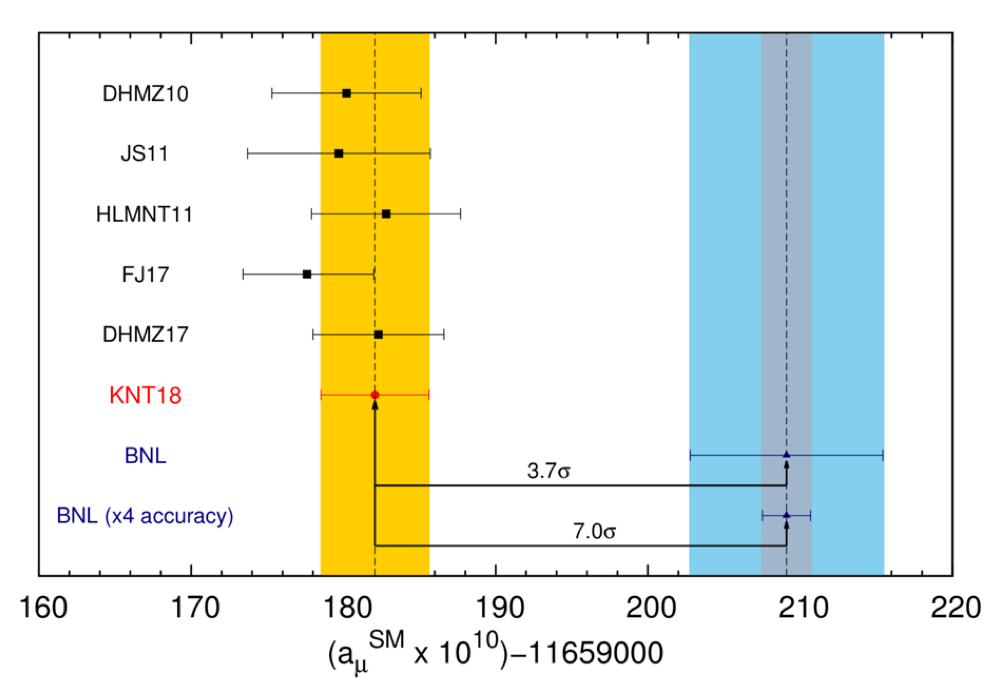
\includegraphics[width=0.9\textwidth]{AlexKPaperComparison}
	\caption[Comparison between theoretical and experimental values for \amu]{Various theoretical values for \amu on the left, as compared to the most recent and extrapolated experimental result on the right. Plot courtesy of Alex Keshavarzi \cite{Keshavarzi:2018mgv}.}
	\label{fig:AlexKPaperComparison}
\end{figure}


\section{Experimental value of \amu and discrepancy with \texorpdfstring{$a_{\mu}^{\text{SM}}$}{amusm}}
\label{sec:Background}


The theoretical contributions to \amu listed in the previous sections have improved over time as methods have matured and more experimental data gathered. Similarly, work on the direct experimental measurement of \amu has been going on for decades, with more precise results being determined over time \cite{PastExperiments}. The most recent experiment to measure \gmtwo was the Brookhaven Muon \gmtwo Experiment (E821) held at Brookhaven National Laboratory (BNL) in 2001 \cite{E821FinalReport}. That experiment measured a value for \amu of 
		\begin{align}
            a_{\mu}^{\text{Exp}} = (11659208.0 \pm 6.3) \times 10^{-10},
		\end{align}
which corresponds to a 540 ppb relative uncertainty. Note that the uncertainty of the experimental measurement is comparable to that of the theory, necessitating precise understanding of all the different theoretical parts. The difference between the experimental and theoretical values here is
		\begin{align}
            a_{\mu}^{\text{Exp}} - a_{\mu}^{\text{SM}} = (27.74 \pm 7.25) \times 10^{-10},
		\end{align}
corresponding to a discrepancy of 3.83$\sigma$ from 0.



\textbf{-double check the numbers here later on down the line, values like \amu experimental may even have changed if other constants have changed}




\section{Beyond the Standard Model and the purpose of E989}
\label{sec:BSM}


While the discrepancy between experiment and theory might be attributed to miscalculations in the theory or systematic errors in the E821 experiment, no such errors have been found despite serious attempts to resolve the two. Indeed the discrepancy has only grown over time as the theoretical calculations have matured. The most intriguing and exciting source of the discrepancy would be physics beyond the standard model (BSM). Since the value of \amu receives contributions from all particles that couple to the muon through virtual loops, unknown particles might be the source of this discrepancy. Specifically, since the contribution to the magnetic moment from heavy virtual particles goes as 
		\begin{align}
            a \sim \frac{m^{2}}{\Lambda^{2}},
		\end{align}
where $\Lambda$ is the mass scale of the new particle and m the mass of the lepton in question, the sensitivity of the muon as compared to the electron to large mass scales is $ m_{\mu}^{2} / m_{e}^{2} \approx 43000$ greater. It is possible from this reason that even though the magnetic moment of the electron has been measured extraordinarily precisely, to .23 ppb \cite{ElectronMDM,CODATA}, it has provided no indication of anything new, whereas the magnetic moment of the muon might provide definitive evidence of new physics.

A basic example diagram of new physics is shown in \figref{fig:BSM}. Because the discrepancy from the previous experiment was not at the 5$\sigma$ level necessary to classify it as a discovery, the E989 experiment was undertaken. Indeed with the lack of new physics results coming out of the LHC and other experiments, E989 is especially positioned to uncover something new at a time where there are so few hints of new physics. Because of this, the interest in the E821 experiment and underway E989 experiment has only grown over time. The number of citations for the E821 results has been consistently high over the years and is shown in \figref{fig:E821Citations}.

\begin{figure}[]
\centering
	\begin{tikzpicture}[baseline=(o.base)]
	\begin{feynhand}
	\large
	\setlength{\feynhandlinesize}{1pt}
	\vertex [ringblob] (o) at (0,0) {BSM};
	\vertex (a) at (-2,-2) {$l$}; 
	\vertex (b) at (2,-2) {$l$}; 
	\vertex (c) at (0,2) {B};
	\propag [fermion] (a) to (o);
	\propag [anti fermion] (b) to (o);
	\propag [photon] (c) to [edge label = $\gamma$] (o);
	\end{feynhand}
	\end{tikzpicture}
\caption[Example diagram for new physics]{An example Feynman diagram, where the leptons couple to an external magnetic field B through some BSM physics. Feynman diagrams made with \cite{tikz-feynman,tikz-feynhand}.}	
\label{fig:BSM}
\end{figure}

\begin{figure}[]
	\centering
	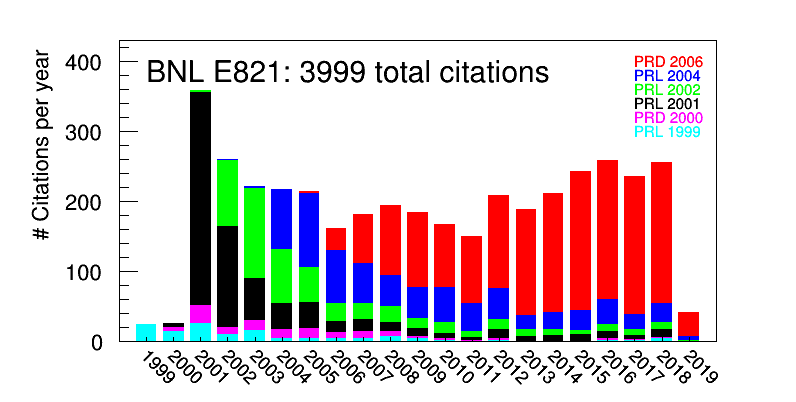
\includegraphics[width=0.9\textwidth]{E821Citations}
	\caption[Citations for E821 publications vs year]{The number of citations for the BNL experiment publications as a function of year. Plot courtesy of Mark Lancaster. \textbf{Update this plot before submission.}}
	\label{fig:E821Citations}
\end{figure}


The E989 experiment has the goal of measuring \amu to 140 ppb over the course of several years. This would be a factor of 4 improvement over the E821 result stemming from a 20 times increase in statistics, which was the limiter in the previous experiment. Assuming the same value for \amu is measured, this would push the discrepancy over the 5$\sigma$ mark to approximately 7$\sigma$, as shown in \figref{fig:AlexKPaperComparison}. The data comprising Run 1, gathered in the spring and summer of 2018, is the subject of this thesis, and corresponds to an experimental uncertainty comparable to the E821 result. When it's all said and done, the possibility is that we will measure something new and exciting, pushing the discrepancy out beyond the 5$\sigma$ level. Even if we do not however, it is valuable in itself to resolve this theoretical and experimental conflict.




% \subsection{Why the muon and not the electron?}

% The magnetic dipole moment of the electron has been measured extraordinarily precisely, to .28 parts per trillion (ppt) \cite{ElectronMDM}. It has been used to test SM theory extensively, and specifically the QED portion of it. Because the electron is so light, the contributions to $a_{e}$ come almost exclusively from QED. This is because the various contributions from both the weak and hadronic sectors contain couplings which depend on the mass of the particle squared. It is for this reason that the magnetic moment of the muon is such an interesting quantity to measure. Since the muon is approximately 200 times heavier than the electron, the senstivity of \amu to radiative corrections is approximately 40000 times greater than that for the the electron.

















\cleardoublepage

%!TEX root = ../thesis.tex

\thispagestyle{myheadings}

\graphicspath{{Body/Figures/ExperimentalOverview/Decay/}{Body/Figures/TrackingFigures/TrackerPics/}{Body/Figures/ExperimentalOverview/Ring/}{Body/Figures/ExperimentalOverview/Auxiliary/}}

\chapter{Principle Technique of E989}
\label{chapter:E989}

As referenced in \equref{eq:torque}, a particle in a magnetic field will experience a torque which attempts to line up the magnetic dipole moment of the particle with the external field. Because of this, in a dipole field a particles spin will turn at the Larmour precesssion frequency \cite{Jackson}
        \begin{align} \label{eq:ws}
            \vec{\omega}_{s} = -g\frac{q}{2m}\vec{B} - (1-\gamma)\frac{q}{\gamma m}\vec{B},
        \end{align}
where as before $m$ is the particles mass, $q = \pm e$ where $e$ is the elementary charge, \g is the g-factor, $\gamma$ is the Lorentz relativistic factor, and $B$ is an external magnetic field. The second term is a relativistic correction to the precession frequency called Thomas precession \cite{Jackson}. Similarly, a particle with some momentum will orbit at the cyclotron frequency
        \begin{align} \label{eq:wc}
            \vec{\omega}_{c} = -\frac{q}{\gamma m}\vec{B}.
        \end{align}
By taking the difference between these two frequencies we arrive at the "spin difference frequency"
        \begin{align} \label{eq:wasimple}
            \vec{\omega}_{a} = \vec{\omega}_{s} - \vec{\omega}_{c} = -\frac{g-2}{2}\frac{q}{m}\vec{B} = - a \frac{q}{m}\vec{B},
        \end{align}
a frequency that is directly proportional to the anomalous magnetic moment $a$. Briefly note that if $g = 2$ as in a Dirac theory, then the particles spin would turn at the same rate as the momentum vector, and this spin difference frequency \wa would be identically 0. If this spin difference frequency for a muon and the external magnetic dipole field can be measured, then the anomalous magnetic moment of the muon \amu can be measured. Introductory descriptions for both will be given here, while the details are left to \chapref{chapter:SpinPrecessionMeasurement} and 
\chapref{chapter:MagneticFieldMeasurement} respectively.


\section{Measuring \texorpdfstring{\wa}{wa}}
\label{section:WaIntro}

How can \wa for muons be measured? The answer lies with two key points in the dynamics of muon decay. Positive muons decay to a positron and two neutrinos, as shown in \figref{fig:mudecay}. The first point is that because of the parity violating nature of the weak interaction, the decay positron will be preferentially emitted right-handed, with its spin directed in the same direction as its momentum \cite{Bucksbaum}. The second key point is that angular momentum must be conserved. Consider the most extreme examples of maximum and minimum energy positrons as shown in \figref{fig:MuonDecayImproved}. In the muon rest frame, decay positrons with maximum energy will be emitted opposite to the two neutrinos. Since neutrinos and anti-neutrinos must be left and right-handed respectively, thus having their spins anti-parallel and parallel to their momentum, by the law of conservation of angular momentum the positron must have its spin be parallel to the spin of the muon at the time of the decay. By the opposite argument, decay positrons emitted with minimum energy such that the neutrinos are ejected opposite to one another must have their spins be anti-parallel to that of the muon at the time of decay. These two points combined together means that higher energy decay postrons will preferentially be emitted in directions parallel to the muon spin at the time of decay, while lower energy decay positrons will preferentially be emitted in directions anti-parallel to the muon spin at the time of the decay. 

\begin{figure}[]
\centering
    \subcaptionbox{$\mu^{+}$ decay through a $W^{+}$ boson to a positron, muon anti-neutrino, and an electron neutrino. This is the dominant decay mode.
    \label{fig:mudecay}}
    {
    \centering
        \begin{tikzpicture}[baseline=(o.base)]
        \begin{feynhand}
        \large
        \setlength{\feynhandlinesize}{1pt}
        \vertex [dot] (o) at (0,0);
        \vertex (a) at (-2,0) {$\mu^{+}$}; 
        \vertex (b) at (1.5,1.5) {$\overline \nu_{\mu}$}; 
        \vertex (c) at (1.5,-1.5);
        \vertex (d) at (3,0) {$\nu_{e}$};
        \vertex (e) at (3,-3) {$e^{+}$};
        \propag [anti fermion] (a) to (o);
        \propag [fermion] (b) to (o);
        \propag [boson] (o) to [edge label' = $W^{+}$] (c);
        \propag [fermion] (c) to (d);
        \propag [anti fermion] (c) to (e);
        \end{feynhand}
        \end{tikzpicture} 
    }
    \hspace{10mm}
    \subcaptionbox{$\pi^{+}$ decay through a $W^{+}$ boson to a $\mu^{+}$.
    \label{fig:pidecay}}
    {
    \centering
        \begin{tikzpicture}[baseline=(o.base)]
        \begin{feynhand}
        \large
        \setlength{\feynhandlinesize}{1pt}
        \vertex [dot] (o) at (0,0);
        \vertex (a) at (-1.5,1.5) {$u$}; 
        \vertex (b) at (-1.5,-1.5) {$\overline d$}; 
        \vertex (c) at (2,0);
        \vertex (d) at (3.5,1.5) {$\mu^{+}$};
        \vertex (e) at (3.5,-1.5) {$\nu_{\mu}$};
        \propag [fermion] (a) to (o);
        \propag [anti fermion] (b) to (o);
        \propag [boson] (o) to [edge label = $W^{+}$] (c);
        \propag [anti fermion] (c) to (d);
        \propag [fermion] (c) to (e);
        \end{feynhand}
        \end{tikzpicture}  
    }
\caption[Feynman diagrams for muon and pion decay]{Feynman diagrams for muon (left) and pion (right) decay.}    
\label{fig:DecayDiagrams}
\end{figure}

\begin{figure}[]
    \centering
    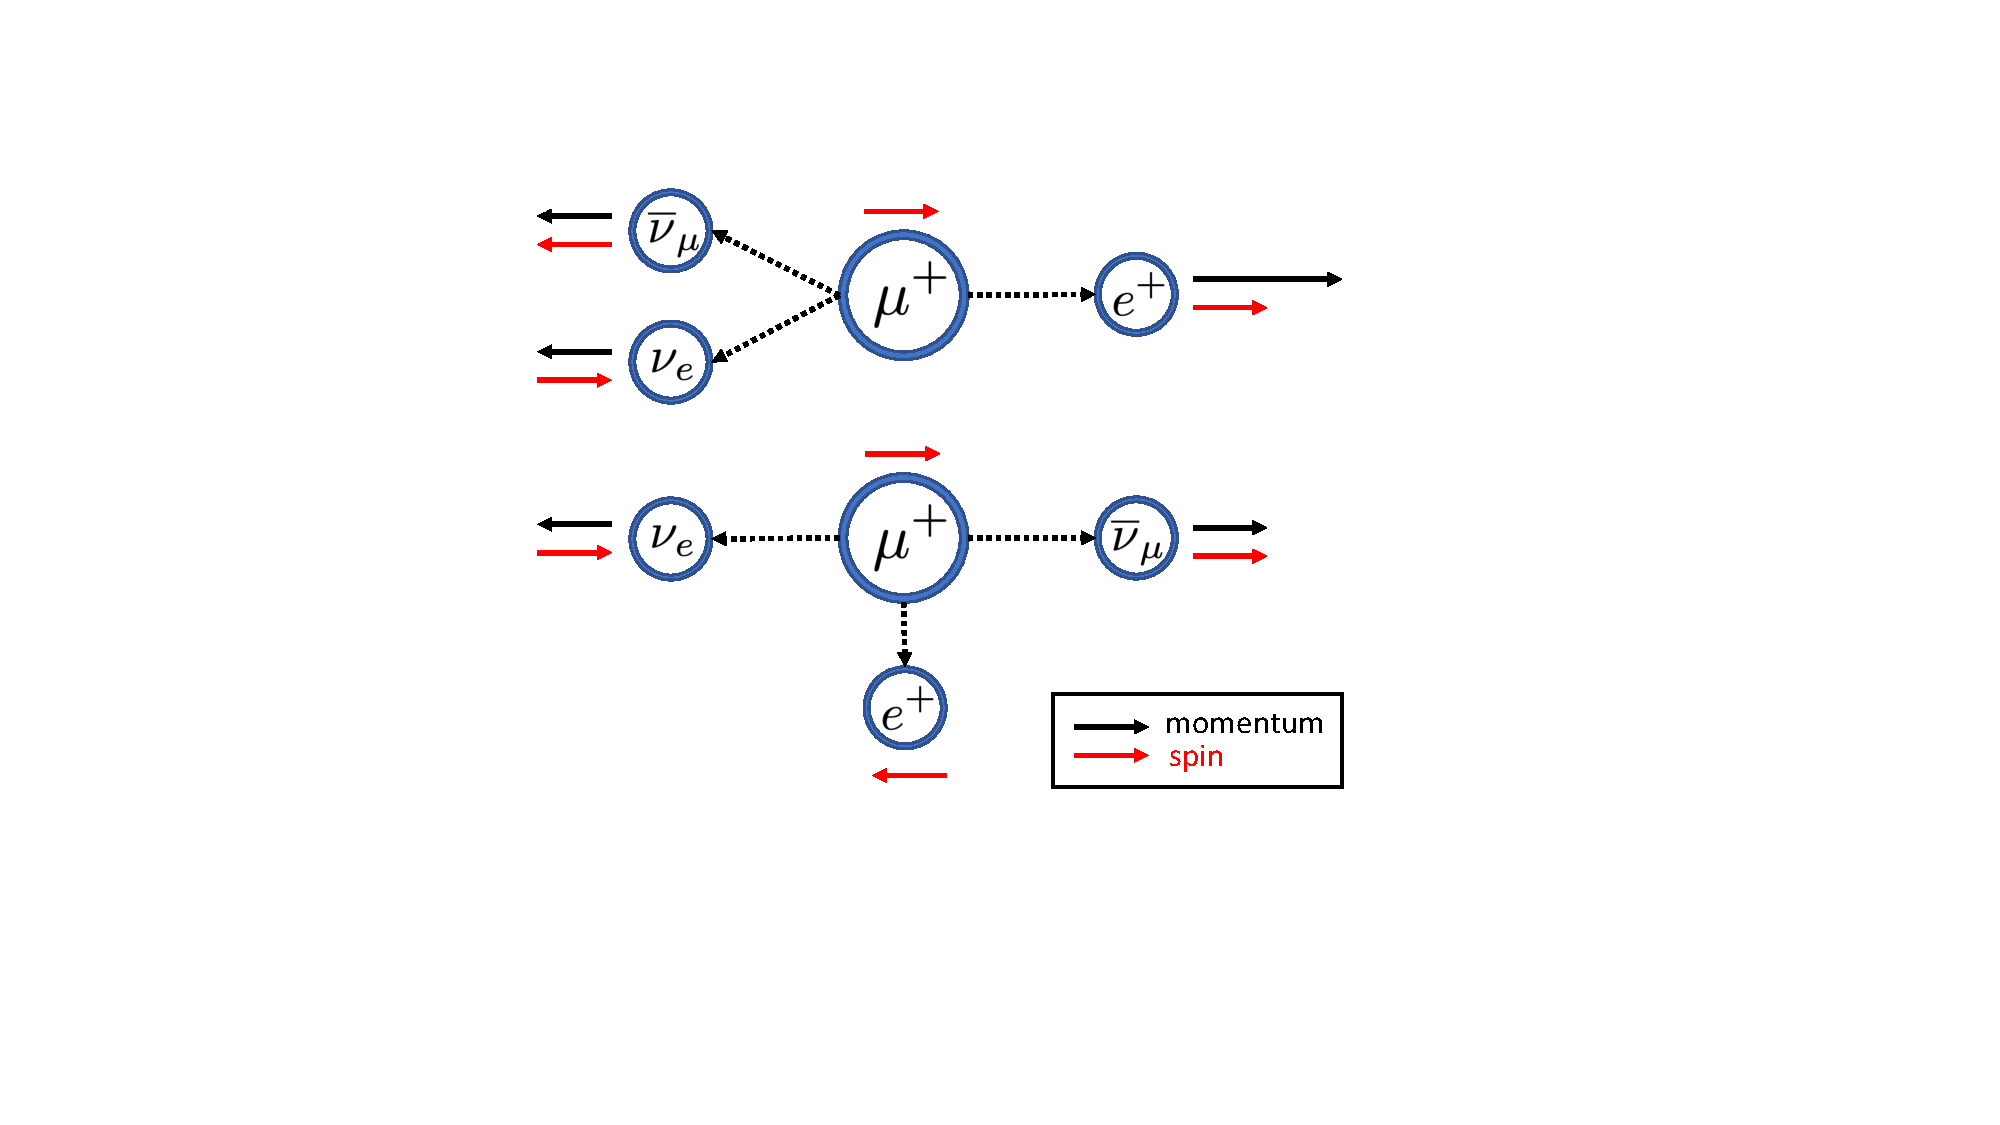
\includegraphics[width=0.6\textwidth]{MuonDecayImproved}
    \caption[Muon decay pictures for maximum and minimum energy decay positrons]{Muon decay pictures for maximum and minimum energy decay positrons. Due to the conservation of angular momentum and the single possible helicity states of the decay neutrinos, the spin of the decay positron is exactly parallel to the spin of the muon at the time of the decay for maximum energy decay positrons (top), or anti-parallel for minimum energy decay positrons (bottom).}
    \label{fig:MuonDecayImproved}
\end{figure}


This correlation between the emitted direction of the decay positron and the spin of the muon is the signature needed to measure \wa. By placing an ensemble of polarized muons within a magnetic storage ring, those muons will orbit at the cyclotron frequency and their spins will precess at the Larmour frequency. As they go around the ring they will decay to positrons whose energy and decay directions contain information about the spin of the muon. The differential decay distribution in the muon rest frame is described by \cite{Bucksbaum}
        \begin{align} \label{eq:diffdecaydist}
            dP(y, \theta) \propto N(y)[1 \pm A(y)\cos(\theta)]dy d\Omega,
        \end{align}
where $y=E/E_{max}$ is the energy fraction of the positron, $\theta$ is the angle between the spin of the muon and the momentum of the positron $\cos^{-1}(\hat{p} \cdot \hat{s})$, and the $\pm$ stands for the positive and negative muon respectively. $N(y)$ is the number distribution of decay positrons and $A(y)$ is the so called 'asymmetry' encoding the preferred positron decay direction. Here the energy of the positron is assumed to be much greater than its mass. The number distribution and asymmetry are given by \cite{Bucksbaum}
        \begin{align}
            N(y) &= 2y^{2}(3-2y^{2}), \label{eq:Nmrf} \\
            A(y) &= \frac{2y-1}{3-2y}, \label{eq:Amrf}
        \end{align}
and are shown in \figref{fig:NA2mrf}. 

\begin{figure}[]
\centering
    \begin{subfigure}[]{0.45\textwidth}
        \centering
        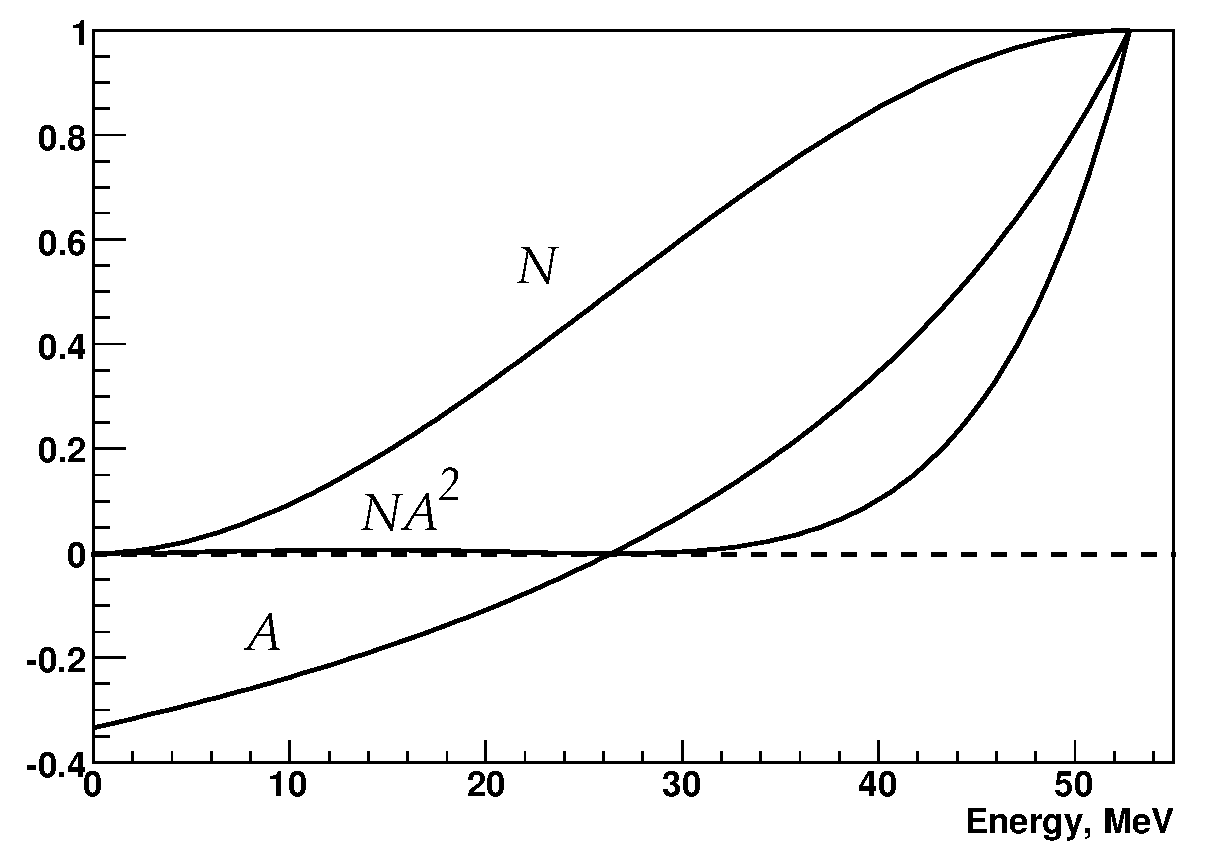
\includegraphics[width=\textwidth]{NA_mrf}
        \caption{Muon rest frame}
    \label{fig:NA2mrf}
    \end{subfigure}%
    \hspace{1cm}
    \begin{subfigure}[]{0.45\textwidth}
        \centering
        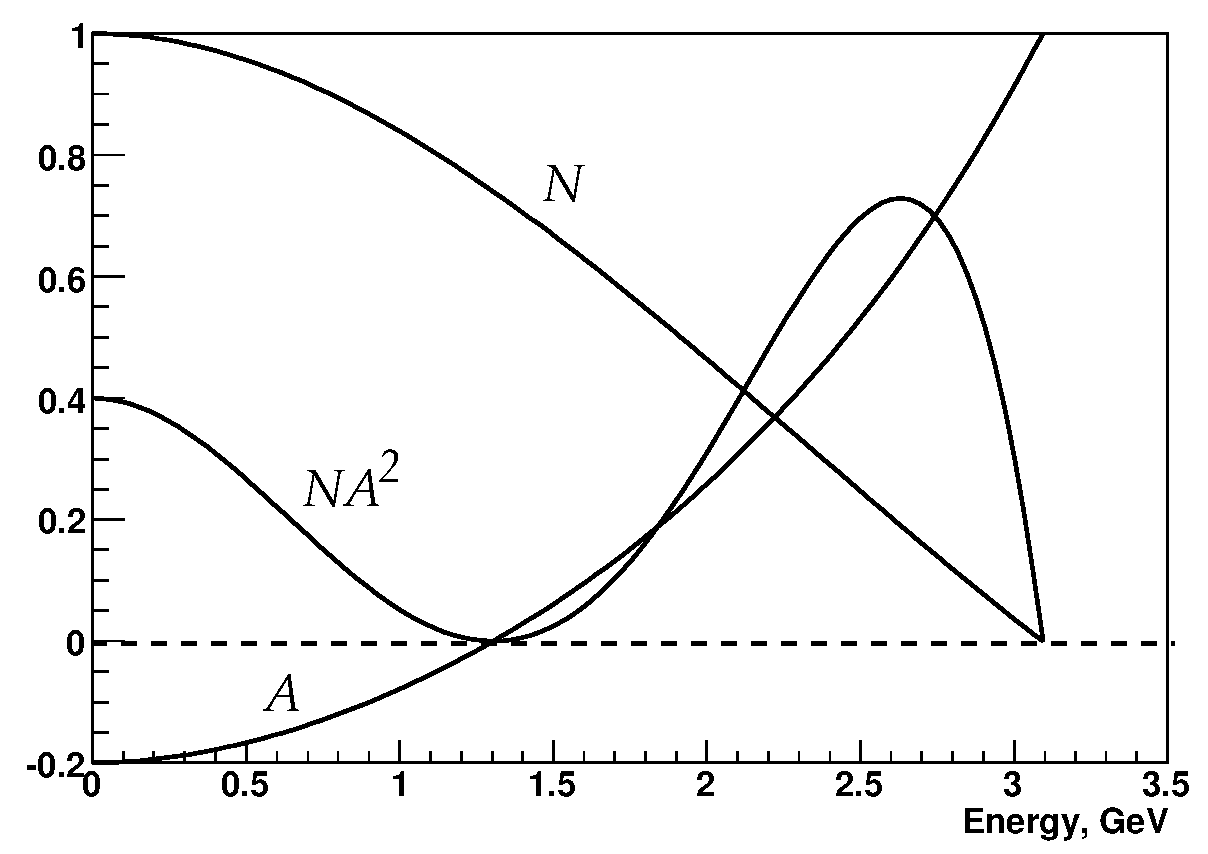
\includegraphics[width=\textwidth]{NA_lab}
        \caption{Lab frame}
    \label{fig:NA2lab}    
    \end{subfigure}
\caption[Number distribution and asymmetry for muon decay in the muon rest frame and lab frame]{Decay number distribution $N$ and asymmetry $A$ in the muon rest frame (left) and in the lab frame (right) as a function of positron energy with a maximum positron energy of 3.1 \GeV.}
\label{fig:NA2}
\end{figure}

In the lab frame for high energy positrons, nearly all positrons will be emitted parallel to the muon momentum, which makes it challenging to select purely on the decay angle of the positron. That's not a problem though, as we already know that decay positrons with higher energies will be emitted in directions parallel to the muon spin at the time of decay. Essentially, the energy distribution of detected positrons for high energies is modulated by \wa, or $\theta = \omega_{a}t + \phi$. The number of detected positrons at some time and energy in the lab frame for some initial number $N_{0}$ of muons can then be described by
        \begin{align}
            N_{d}(t, E) = N_{0}(E) \cdot e^{-t/\gamma\tau_{\mu}} \cdot [1 + A(E) \cos(\omega_{a}t+\phi(E))],
        \end{align}
where the $d$ subscript stands for 'detected,' the muons are decaying at a lifetime of $\gamma\tau_{\mu}$, and all the relevant parameters are energy dependent. Here $N_{0}(E)$ and $A(E)$ have been transformed from Equations~\ref{eq:Nmrf} and \ref{eq:Amrf} to the lab frame,
        \begin{align}
            N_{0}(E) &\propto (y-1)(4y^{2}-5y-5), \label{eq:Nlab} \\
            A(E) &= \frac{-8y^{2}+y+1}{4y^{2}-5y-5}, \label{eq:Alab}
        \end{align}
where as a reminder $y=E/E_{max}$. Here the polarization of the muons is assumed to be unity. These are shown in \figref{fig:NA2lab}. To increase the amount of statistics, all positrons above some energy threshold cut $E_{th}$ can be taken as the observable,
        \begin{align} \label{eq:5parfunc}
            N_{d}(t, E_{th}) = N_{0}(E_{th}) \cdot e^{-t/\gamma\tau_{\mu}} \cdot [1 + A(E_{th}) \cos(\omega_{a}t+\phi(E_{th}))],
        \end{align}
where the number and asymmetry of the detected positrons is now calculated by simply integrating Equations~\ref{eq:Nlab} and \ref{eq:Alab} from $y_{th}$ to 1,
        \begin{align}
            N_{0}(E_{th}) &\propto (y_{th}-1)^{2}(-y_{th}^{2}+y_{th}+3), \label{eq:Nth} \\
            A(E_{th}) &= \frac{y_{th}(2y_{th}+1)}{-y_{th}^{2}+y_{th}+3}, \label{eq:Ath}
        \end{align}
where $y_{th}=E_{th}/E_{max}$. By fitting \equref{eq:5parfunc}, \wa can be extracted.



\clearpage






\clearpage



In the presence of an electric field, which is useful in storing the muon beam within a dipole magnetic field, this expands to 
        \begin{align} \label{eq:waelectric}
            \vec{\omega}_{a} = -\frac{Qe}{m} [a_{\mu}\vec{B} - (a_{\mu} - \frac{1}{\gamma^{2}-1})(\vec{\beta} \times \vec{E}) ],
        \end{align}
where now the measurable quanties are vector quantities. Finally, for realistic cases of muon momentum which is non-orthogonal to the magnetic field, the spin difference frequency becomes
        \begin{align} \label{eq:wafinal}
            \vec{\omega}_{a} = -\frac{Qe}{m} [a_{\mu}\vec{B} - a_{\mu} (\frac{\gamma}{\gamma+1})(\vec{\beta} \cdot \vec{B})\vec{B} - (a_{\mu} - \frac{1}{\gamma^{2}-1})(\vec{\beta} \times \vec{E}) ].
        \end{align}
If the motion of the muons is largely perpendicular to the magnetic field, then the second term is small and can be corrected for. If the particles have a momentum of approximately 3.09 \GeV/c, the so called ``magic momentum,'' then the third term is small and can be corrected for. These will be talked about later.

In order to measure the spin difference frequency of the muon, a clever technique is used. Decay muons in the pion rest frame are 100\% polarized due to conservation of angular momentum and the fact that the decay neutrino must have a specific helicity. Within a pion beam then the highest and lowest energy decay muons are polarized. Muons will decay to positrons with a lifetime of about 2.2 $\mu$s, and the positrons with the highest energies will be correlated with the muon spin, a so called ``self-analyzing'' decay. The single available decay state for a maximum energy positron illustrates this in \figref{fig:MuonDecay}. Thus, by aquiring a large sample of polarized muons and injecting them into a storage ring 









\begin{figure}[]
    \centering
    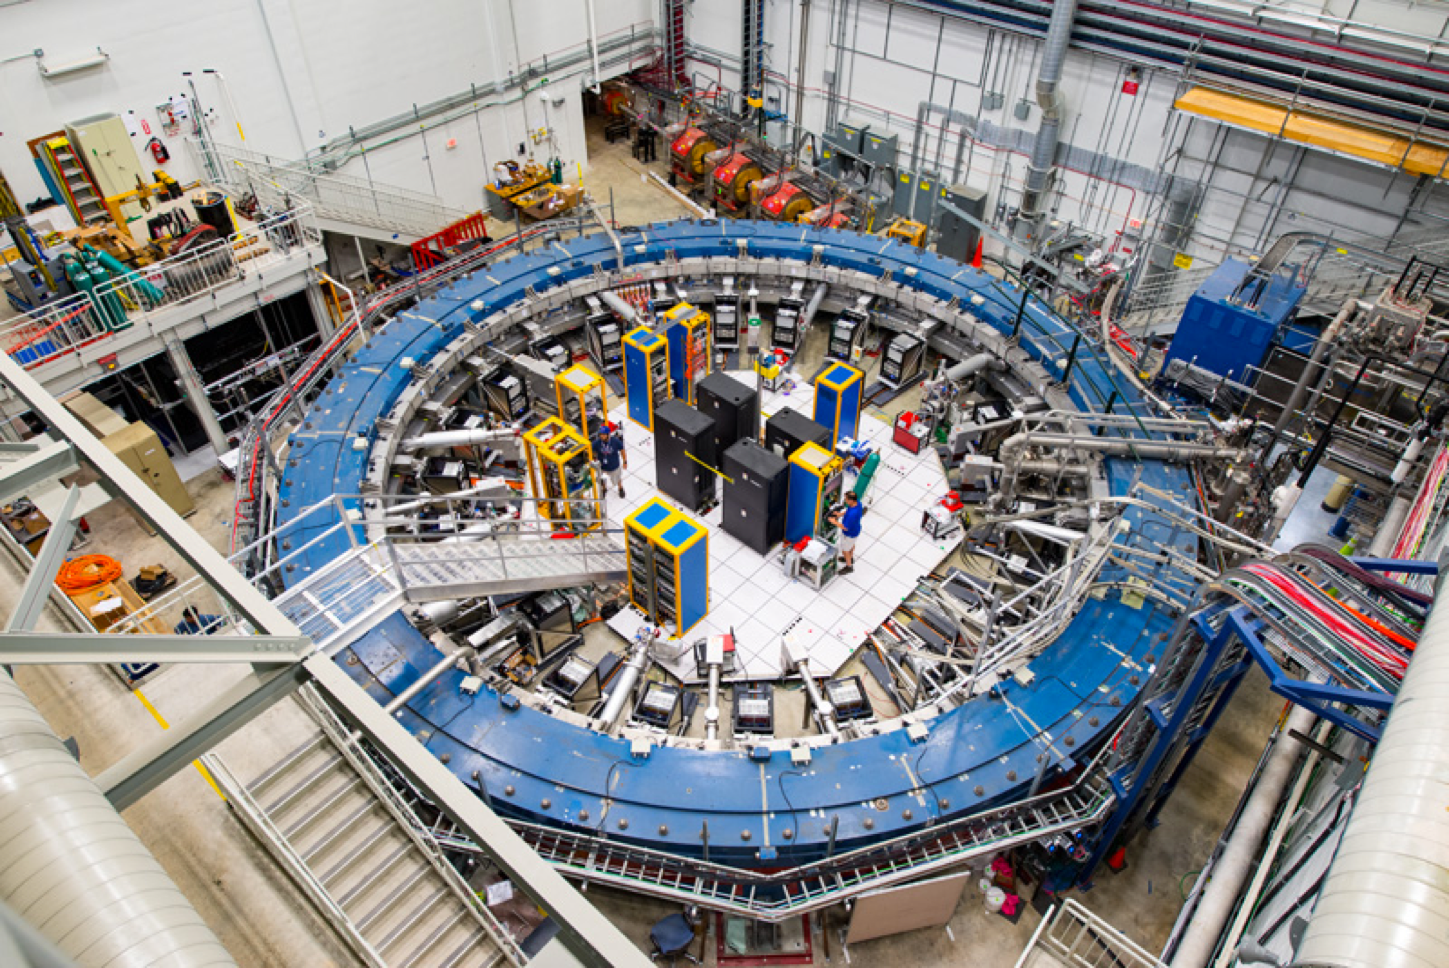
\includegraphics[width=0.9\textwidth]{ring}
    \caption[ring]{clean up and possibly replace}   
    \label{fig:ring}
\end{figure}





\section{Measuring B}
\label{sec:BIntro}






\section{Accelerator}
\label{sec:Accelerator}




\cite{Stratakis:2017uci}


\section{Injection}
\label{sec:Injection}

the inflector



\section{Storage}
\label{sec:Storage}

kickers and quads





\cleardoublepage

%!TEX root = ../thesis.tex

\thispagestyle{myheadings}

\chapter{Magnetic Field Measurement}
\label{chapter:MagneticFieldMeasurement}




Instead of having a overall field chapter, either remove it entirely or dedicate it to the opera simulations I did and the magnetic field measurements I made.




\section{Opera Simulations}
\label{sec:OperaSimulations}







\cleardoublepage

%!TEX root = ../thesis.tex

\thispagestyle{myheadings}

\graphicspath{{Body/Figures/TrackingFigures/}{Body/Figures/TrackingFigures/MainPlots/}{Body/Figures/TrackingFigures/MainPlots/PlanePlots/}{Body/Figures/TrackingFigures/MainPlots/PullPlots/}{Body/Figures/TrackingFigures/MainPlots/Residuals/}{Body/Figures/TrackingFigures/eLoss/}{Body/Figures/TrackingFigures/CoordSys/}{Body/Figures/TrackingFigures/TrackerPics/}{Body/Figures/TrackingFigures/Field/}{Body/Figures/TrackingFigures/TrackingFlow/}{Body/Figures/TrackingFigures/LeftRight/}{Body/Figures/TrackingFigures/Misc/}{Body/Figures/TrackingFigures/Extrapolation/}{Body/Figures/TrackingFigures/Tracks/}}

\chapter{Track Reconstruction and Analysis}
\label{chapter:TrackReconstruction}

As described in section \ref{sec:StrawTrackers}, the straw trackers are used to provide information about the muon beam, important for the calorimeter \wa analysis, calculating the \wa pitch correction, and determining the spatially weighted magnetic field seen by the muons. The track reconstruction is performed in three stages: First, individual hits in the tracker are grouped into individual tracks in the finding stage. Second, a best trajectory is fit to grouped hits in the fitting stage. Third, the best fit trajectory is extrapolated back to the storage region or forwards to the calorimeter in the extrapolation stage. A fourth refinement stage is planned but not yet implemented, which would add or remove hits in the finding stage based on the results of the fitting and extrapolation stages.


\section{Track Finding}
\label{sec:TrackFinding}

The track finding stage consists of pattern recognition routines in order to group individual hits into separate sets corresponding to individual incident tracks. The general implementation of these pattern recognition routines is relatively straightforward \cite{trackfinding,trackfinding2}. Hits across all modules are grouped in time windows called time islands, with a max width of $\SI{100}{ns}$. Within those time islands hits are then grouped into clusters. Clusters consist of one or two hits for each U or V view per module. As a reminder the U and V views of a module consist of the two U or V layers in that module, \secref{sec:StrawTrackers}. Hits are only clustered if they lie in close proximity in time and space to one another. The spatial constraint is defined as the difference in hit straw numbers, from 0 to 31 for the 32 straws per layer, which by default is limited to less than or equal to 4. Neighboring hit clusters in the same module are then grouped to form seeds, one per module. Finally, seeds in successive modules are grouped starting from one end of the tracker to form what are called track candidates. The seeds are formed and grouped into track candidates again only if they lie close in time and space to one another. The entire track candidate formation process occurs for all hits in a time island to find as many real tracks as possible. See \figref{fig:TrackCandidateSelection}.

After a track candidate has been formed a number of checks are made before passing it on to the fitting stage. If hits, clusters, or seeds are found to be shared among multiple track candidates, the candidates are dropped. Likewise, a track candidate is dropped if it is made from seeds consisting of only one type of view, or if the track candidate has less than six hits. There are also various small geometry and timing algorithms to improve the track candidates, such as removing hits from secondaries \cite{trackfinding3}. The $t_{0}$ time for the track candidate is calculated as the mean time of all hits, with some fixed offset at the end. This $t_{0}$ is helpfully constrained by geometry effects, where for a straight track passing through two layers in the same view, the sum of the drift times adds up to a constant (cite or show this?). The track candidate is supplied with an original momentum and position guess at the start of the track by fitting a circle to the hit straw wires in the horizontal plane. The final track candidates are passed on to the fitting stage. 


\begin{figure}[]
    \centering
    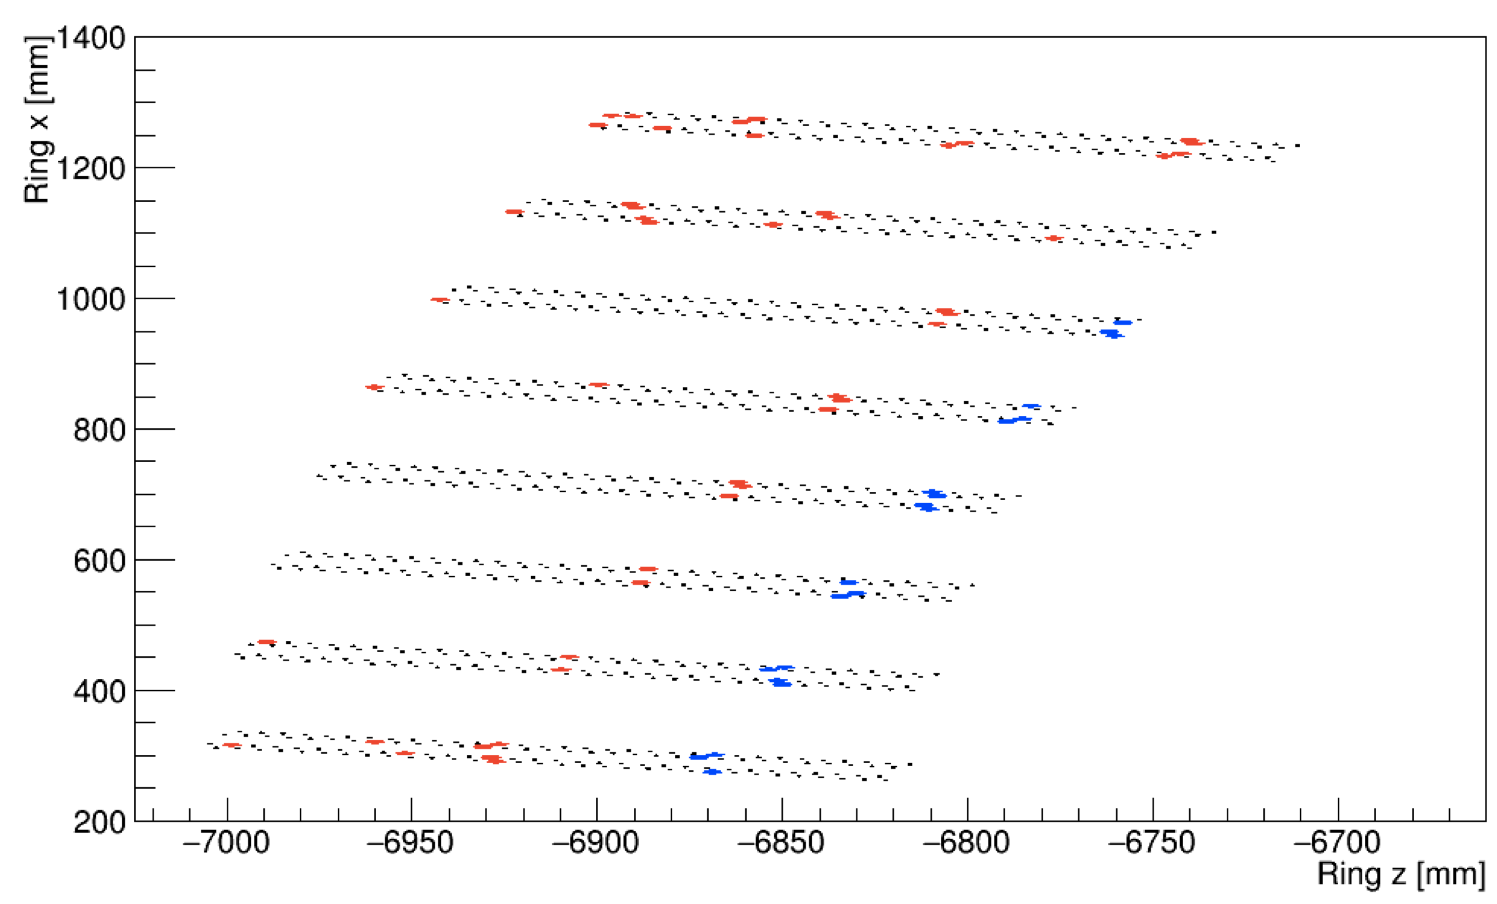
\includegraphics[width=0.9\textwidth]{TrackCandidateSelection}
    \caption[Track candidate selection]{Hits in a tracker station in a single time island. The black dots indicate the position of the straws, while the blue and red points indicate hits. In blue is the first formed track candidate in the island, formed from separate seeds in different modules. The track finding algorithms will move onto the remaining hits in the time island to attempt to form other track candidates, one of which is easily observable by eye.}    
    \label{fig:TrackCandidateSelection}
\end{figure}

% event display tracks

% \begin{figure}[]
% 	\centering
% 	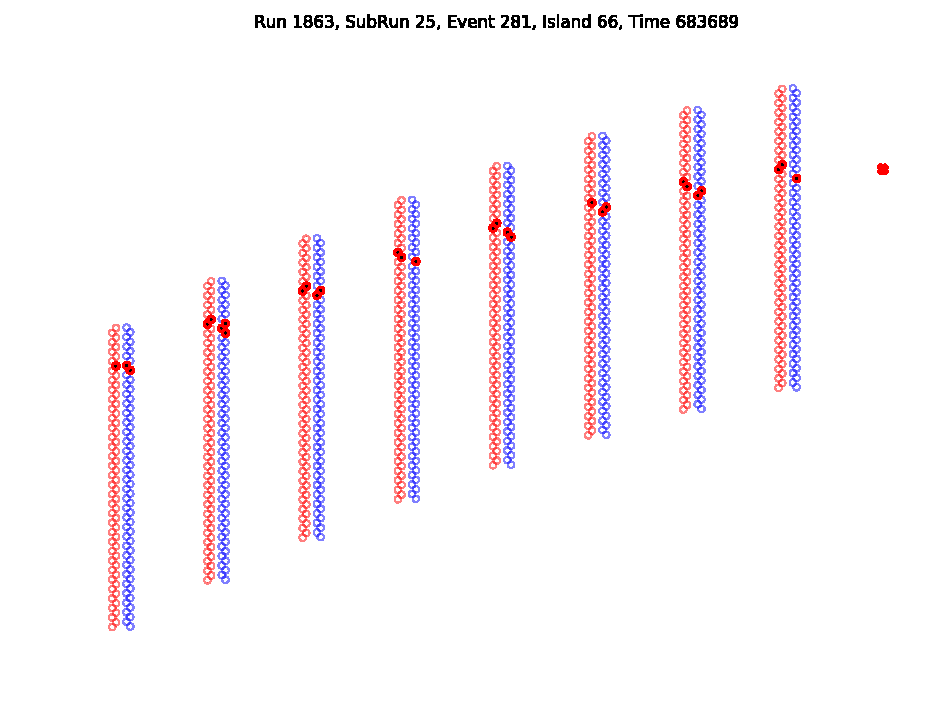
\includegraphics[width=0.9\textwidth]{TrackAndCaloHit}
%     \caption[TrackAndCaloHit]{clean up and possibly replace}    
%     \label{fig:TrackAndCaloHit}
% \end{figure}

% \begin{figure}[]
% 	\centering
% 	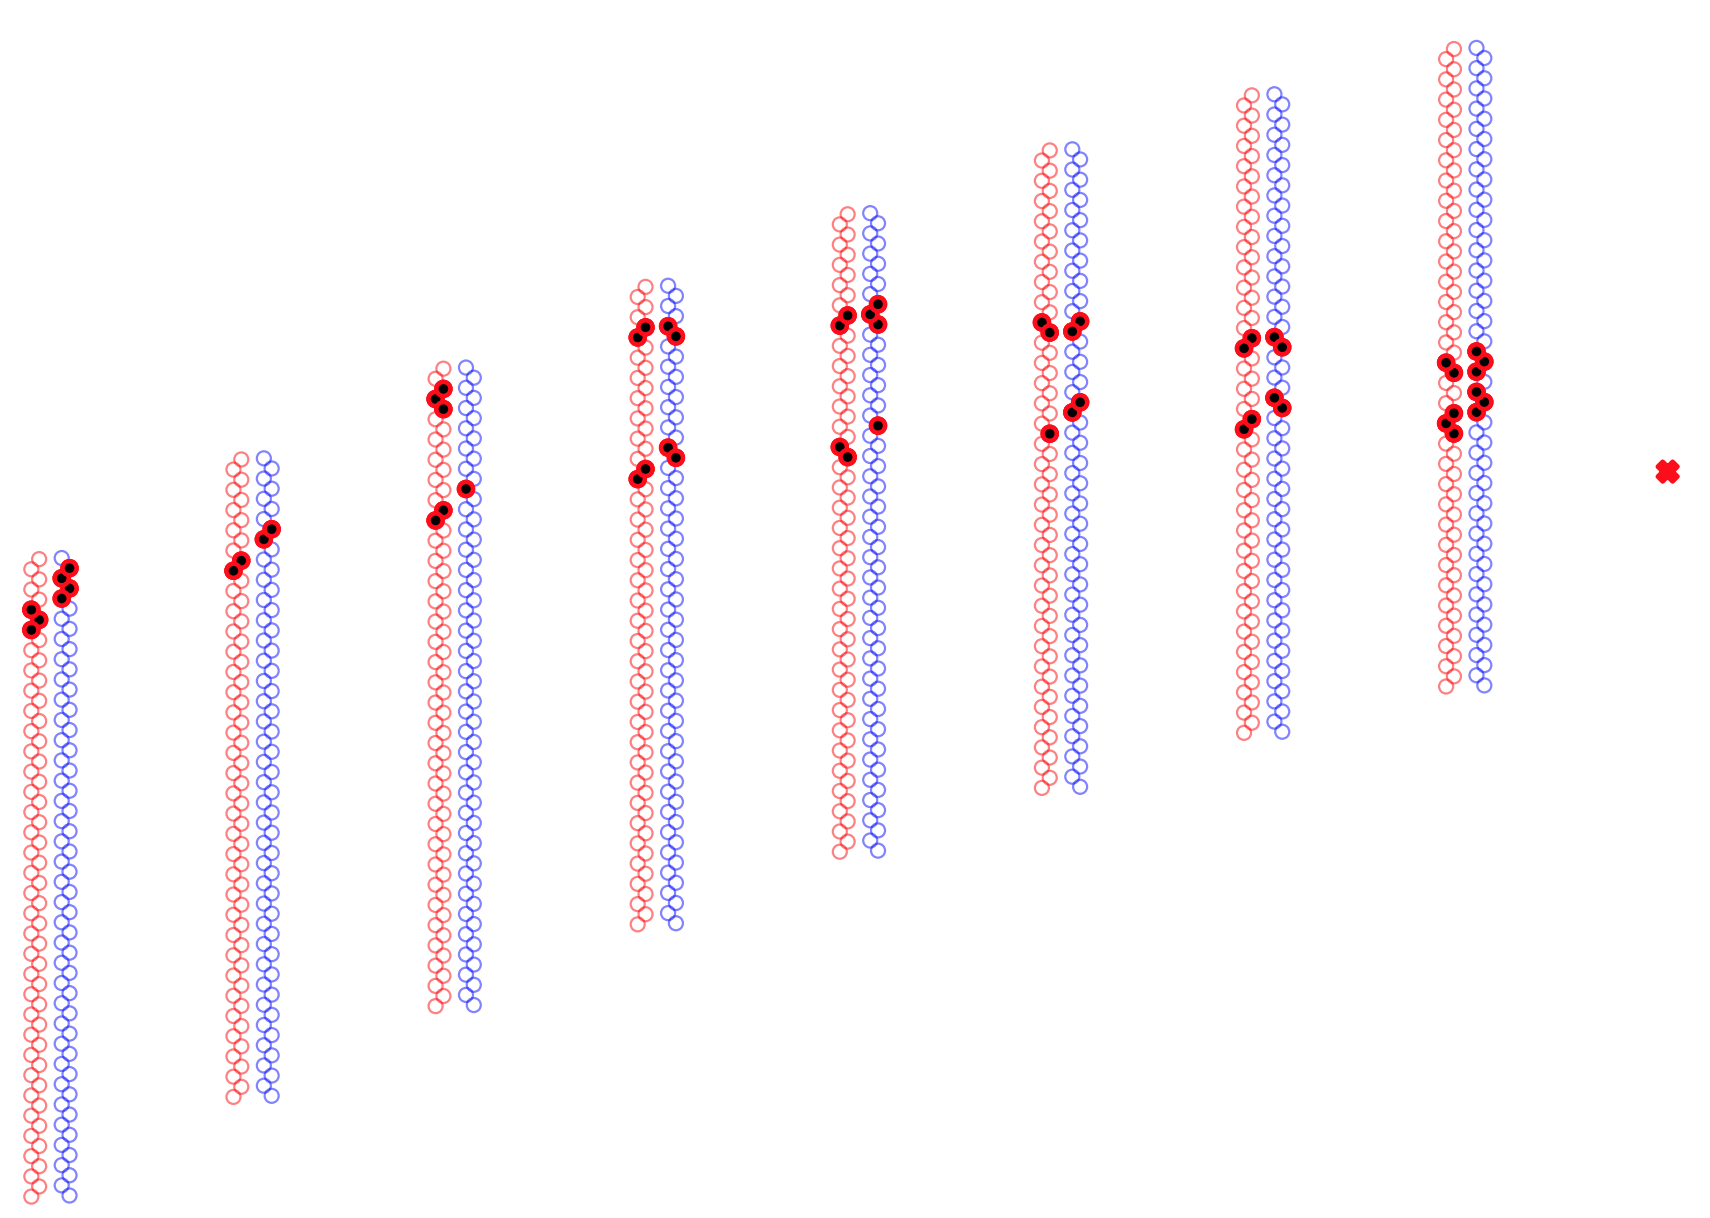
\includegraphics[width=0.9\textwidth]{pileupEvent}
%     \caption[pileupEvent]{clean up and possibly replace}    
%     \label{fig:pileupEvent}
% \end{figure}





\section{Track Fitting}
\label{sec:TrackFitting}


-Geane (Geometry and Error Propagation)


From NIM section I wrote:
The track fitting stage is based off of the GEANE method (Geometry and Error Propagation), that was used successfully in E821 \cite{geanemanual}. A set of track hits  Track defining objects such as transport matrices, error matrices, and predicted parameter vectors are generated within the full g-2 Geant4 simulation from initial guesses. This has the advantage of direct access to both the geometry and material of the trackers as well as the field that the decay positrons experience as they curl inward. This is important as the tracker lives in a region of high field non-uniformity as shown in Figure~\ref{fig:operaBy}. These track objects are then plugged into a global chi-squared minimization algorithm which produces an optimal state vector near the start of the tracker. This minimization is performed in the same reference frame as the tracker measurement frame, which reduces parameter correlations and improves the fitting. The final state vectors are then passed to the extrapolation stage.






The Geane fitting routines originated in Fortran with the EMC collaboration, and was used in the precursor E821 experiment as well as the PANDA experiment with some success \cite{geanemanual}, \cite{Lavezzi}. (I'm not actually aware of a useful reference for it's use in E821, and there are some other instances of its use as well in other experiments. In E821 there was a single tracking chamber which was never put to full use.) The core error propagation routines were at some point added to Geant4 under the error\_propagation directory which is included in all default installs. The tracking code strengths lie with its direct implementation and access to the Geant4 geometry and field, and its ability to handle the field inhomogeneities. The Geane fitting algorithm code which makes use of the Geant4 error propagation routines follows the structure of \cite{geanemanual} and is detailed in the \hyperref[sec:Formalism]{Formalism} section in this paper. It is a relatively straight forward least squares global \chisq minimization algorithm. 


Because of the proximity of the trackers to the muon beam, they will lie within a region of varying magnetic field. The radial field of the trackers rises from 0 Tesla at the outer ends to roughly .3 Tesla at the inner top and bottom ends, and the vertical field drops approximately 50\% from the storage dipole field of 1.451 Tesla. Shown in \figref{fig:Opera2DFields} is the location of the tracker with respect to the horizontal and vertical fields. These large field gradients over the tracking detector region and the long extrapolation distance back to the muon decay point are special to Muon \gmtwo. This is one of the main motivations for using the Geane fitting algorithm and routines, which has direct access to the field.

\begin{figure}[]
\centering
    \begin{subfigure}[]{0.75\textwidth}
        \centering
        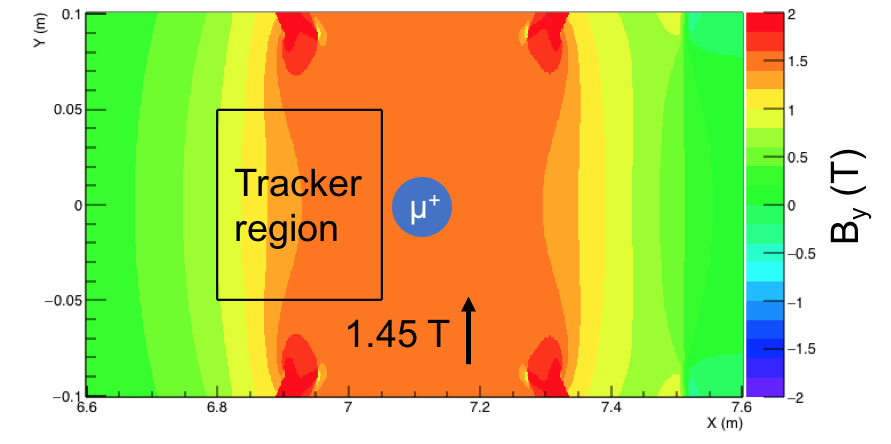
\includegraphics[width=\textwidth]{operaByMod}
        \caption{Vertical magnetic field}
    \label{fig:operaBy}
    \end{subfigure}%
    \vspace{5mm}
    \begin{subfigure}[]{0.75\textwidth}
        \centering
        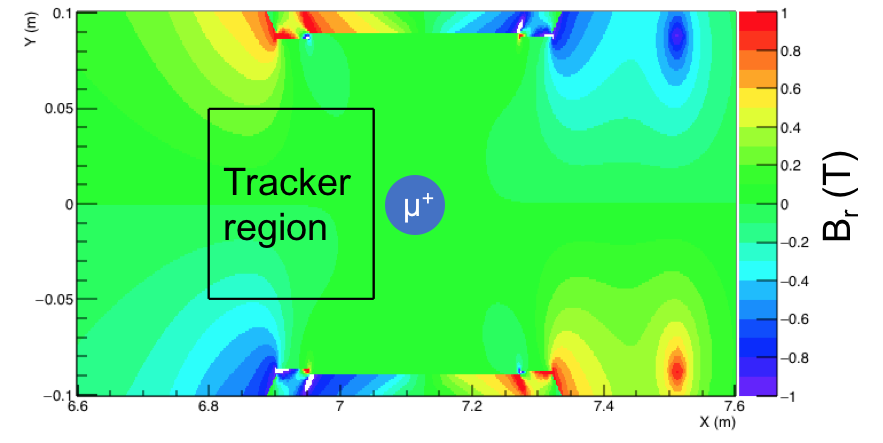
\includegraphics[width=\textwidth]{operaBxMod}
        \caption{Radial magnetic field}
    \label{fig:operaBx}
    \end{subfigure}
\caption[Vertical and radial magnetic fields calculated in Opera2D]{Shown are the vertical (top) and radial (bottom) magnetic fields of the storage ring magnet in and around the storage region as calculated in Opera 2D. The horizontal and vertical axes are the radial and vertical coordinates of the ring respectively. The center of the storage region lies at $\SI{7.112}{m}$ along the horizontal axis. The contours represent the strengths of the vertical and radial magnetic fields. The black box shows the rough location of the tracker with respect to the ring. It can be seen that there is a large field non-uniformity within the tracker space.}
\label{fig:Opera2DFields}
\end{figure}





\subsection{Track Fitting Formalism}
\label{sec:TrackFittingFormalism}

    I recommend reading \cite{geanemanual}, Chapter 4 of \cite{Lavezzi}, and \cite{trajfit} in order to best understand the fitting algorithm. However, due to the at times confusing notation, ommitted equations or concepts, and differences between papers, I have attempted to summarize here the different sources and present the material in a more understandable and readable format. The implementation of the fitting algorithm into the code follows this section.

    One can define a $\chi^{2}$ for a track in the usual way by dividing the residuals of measured and predicted track parameters by their errors:
        \begin{align} \label{eq:chi2}
            \chi^2 = (\vec{p}-\vec{x})^{T} (\sigma^{-1}) (\vec{p}-\vec{x}),
        \end{align}
    where $\vec{p}$ are predicted track parameters from a fit to the measured track parameters $\vec{x}$, and $\sigma$ is a covariance matrix of errors on the fitted parameters. The Geant4 error propagation routines can be used to determine these predicted parameters and error matrices by propagating track parameters from some initial guesses. By minimizing this $\chi^{2}$ with respect to the track parameters one can then fit and improve the track. The Geant4 error propagation routines propagate particles along their average trajectories neglecting the effects of discrete processes, using a helix equation along small enough steps where the change in the magnetic field is small. The predicted parameters are then a function of path length: 
        \begin{align} \label{eq:pp}
            p_{l} = F_{l,l_{0}}(p_{0}),
        \end{align}
    where the path length can be defined how one wishes. In our system we have tracker planes defined at X positions, and limit path lengths to reach those planes. (From here on the dependence on path length or X position will be neglected, in favor of using plane indices.) In tandem, error matrices describing the expected distribution in true parameters about those predicted parameters due to said discrete process are also calculated:
        \begin{align} \label{eq:sigma}
            \sigma^{ij} = <p^{i}p^{j}> - <p^{i}> \cdot <p^{j}>,
        \end{align} 
    where i and j are track parameter indices. These parameter vectors are 5x1 objects defined in some track representation, as described in the \hyperref[sec:Coord]{Coordinate Systems} section. The propagation of these parameters and error matrices are done using transport matrices, which express the infinitesimal changes in parameters at some plane (or path length) with respect to the parameters at some previous plane (or previous path length):
        \begin{align} \label{eq:transport}
            \delta p_{N} &= T_{N,N-1} \delta p_{N-1}, \\
            \sigma_{N} &= T_{N,N-1} \sigma_{N-1} T_{N,N-1}^{T}.
        \end{align}
    Said transport and error matrices are 5x5 objects since the parameter vectors are 5x1 objects as described above. The calculation of these transport matrices, as well as details on the functional form of \ref{eq:pp} are shown in \cite{jacob}.

    With parameters defined on such planes, one can define the $\chi^{2}$ as: 
        \begin{align} \label{eq:chi2sum}
            \chi^2 = \sum_{i=1}^{N} [(p_{i}(p)-x_{i})^{T} (\sigma_{i}^{-1}) (p_{i}(p)-x_{i})],
        \end{align}
    where $p_{i}$ are the average predicted parameters from some general starting parameters $p$. At first order one can solely include the measurement errors on parameters, which fill in the diagonals of $\sigma_{i}$, if random processes can be neglected. Unmeasured parameters should have measurement errors of infinity (or some large value) along the diagonals in the code, which account for the fact that residuals for unmeasured parameters do not exist. When the error matrix is inverted all rows and columns of the matrix with these large numbers will fall to 0 in the $\chi^{2}$. 

    In order to get the best fit track, the $\chi^{2}$ should be minimized with respect to the initial track parameters p, and evaluated at some chosen or fitted parameters:
        \begin{align} \label{eq:minimize}
            \frac{\partial \chi^{2}}{\partial p}|_{p=p'_{0}} = 0,
        \end{align}
    resulting in
        \begin{equation}
        \begin{aligned}
            0 = \sum_{i=1}^{N}[ (\frac{\partial p_{i}(p)}{\partial p}|_{p=p'_{0}})^{T} (\sigma_{i}^{-1}) (p_{i}(p'_{0})-x_{i}) \\ 
            + (p_{i}(p'_{0})-x_{i})^{T} \frac{\partial(\sigma_{i}^{-1})}{\partial p}|_{p=p'_{0}} (p_{i}(p'_{0})-x_{i}) \\ 
            +  (p_{i}(p'_{0})-x_{i})^{T} (\sigma_{i}^{-1}) (\frac{\partial p_{i}(p)}{\partial p}|_{p=p'_{0}})]
        \end{aligned}
        \end{equation}
    where the 1st and 3rd terms are identical, and the 2nd term is small if one assumes that the error matrix doesn't change much with respect to the starting parameters. (Fair since most of the error comes from measurement, and as long as the initial guess is decent enough such that the path length through material doesn't change appreciably from one iteration to the next.) This simplifies to: 
        \begin{align} \label{eq:solve}
            \sum_{i=1}^{N} T^{T}_{i0} (\sigma_{i}^{-1}) (p_{i}(p'_{0})-x_{i}) = 0,
        \end{align}
    which is just the top term with 
        \begin{align} \label{eq:transport2}
             T_{i0} = \frac{\partial p_{i}(p)}{\partial p}.
        \end{align}
    To solve this make the substitution 
        \begin{align} \label{eq:psub}
            p_{i}(p'_{0}) = p_{i}(p_{0}) + \frac{\partial p_{i}(p_{0})}{\partial p} \Delta p_{0} = p_{i}(p_{0}) + T_{i0} \Delta p_{0},
        \end{align}
    where $p'_{0}$ are the improved starting parameters for the next iteration calculated from the previous starting parameters $p_{0}$, and $\Delta p_{0}$ are the changes in the starting parameters to improve the track. This equation can be plugged into the above if one makes the assumption that $T_{i0}$ does not change much from one iteration the next, which follows from the inherent nature of making small adjustments to the track in order to improve it.

    After simplifying one arrives at 
        \begin{align} \label{eq:deltap}
            \Delta p_{0} = \sigma_{p_{0}} \sum_{i=1}^{N} T^{T}_{i0}(\sigma_{i}^{-1})(x_{i} - p_{i}(p_{0})),
        \end{align}
    where
        \begin{align} \label{eq:cov}
            \sigma_{p_{0}} = [\sum_{i=1}^{N} T^{T}_{i0} (\sigma_{i}^{-1}) T_{i0} ]^{-1},
        \end{align}
    is the 5x5 covariance matrix of fitted parameters on the starting plane, whose diagonals describe the errors in the 5 track parameters on that plane and in the region close to it. (The fit does not directly return fit errors for track parameters on other planes.) $\Delta p_{0}$ along with $\chi^2$ is exactly what we want to determine since that is what allows us to fit and improve the track from iteration to iteration.

    However, since random processes should not be neglected for optimal tracking results, it makes more sense to return to the original $\chi^2$ in equation \ref{eq:chi2}, only now the included matrix and vector objects are combined into one large linear algebra equation. Instead of a sum over N 5x1 objects multiplying 5x5 error matrices, the vectors are combined into a single 5Nx1 vector multiplying a single 5Nx5N matrix. The 5x5 diagonal blocks of this large error matrix should now include the effects due to material processes as calculated in Geant from equation \ref{eq:sigma} as well as the measurement errors. 

    Because now parameters at one plane are no longer independent of the parameters at other planes, due to correlations from these random processes, it's necessary to add off-diagonal elements into the large error matrix. These 5x5 blocks come from 
        \begin{align} \label{eq:corr}
            \sigma_{MN} = T_{MN} \sigma_{N}, 
        \end{align}
    for the top diagonals, and the transpose for the bottom diagonals, where M and N are two separate planes within the detector. ($\sigma_{N}$ is the error matrix on plane N calculated from the starting plane.) This follows from equation \ref{eq:sigma} evaluated at plane M with respect to a path length from plane N, and not plane 0, which is equivalent to \ref{eq:corr}. 

    You can then minimize the $\chi^{2}$ in the same way, only again with the matrix objects being aggregates of the per plane objects:
        \begin{align} \label{eq:deltafull}
            \Delta \vec{p}_{0} = \sigma_{p_{0}} \tau^{T}\sigma^{-1}(\vec{x}-\vec{p}),
        \end{align}
        %
        \begin{align} \label{eq:covfull}
            \sigma_{p_{0}} = [\tau^{T} \sigma^{-1} \tau ]^{-1},
        \end{align}
    where $\tau$ is the combined transport matrices from the individual 5x5 matrices, a 5Nx5 object.

    The unmeasured parameter errors of infinity still come into play in the final calculation in the same was as before. Because however these matrix objects are very large, and the tracking must have a certain amount of speed in order to keep up with data, it is useful to reduce the size of these matrices. (It also makes things easier programming wise. Note that there are other some other ways to speed things up, specifically the banded inversion method as described in reference \cite{trajfit}. This method was not used in favor of getting the code working in the simpler form in the first place, but it is a possibility in the future to use this technique to speed things up even more.) It suffices to simply remove all rows and columns where said infinity values exist in the error matrix. This is mathematically equivalent to inverting the error matrix with the infinities included, which make all rows and columns where they exist go to zero. The associated unmeasured parameter rows in the residual vector and transport matrices must similarly be removed. This results in an Nx1 residual vector, NxN error matrix, 5xN combined transport matrix transpose, which multiply against the 5x5 covariance matrix out front to still result in a 5x1 fix to the starting parameters, and a scalar $\chi^2$ value. (Note that these element removals should be done just before the final calculation, and not higher up in the algebra, otherwise plane correlations are not properly calculated.)

    By calculating the last two equations one can fit the track, acquire a $\chi^{2}$ describing the degree of the fit, determine how the track parameters can be improved at the starting point, and calculate errors on those starting parameters. This algorithm can be iterated a number of times to get a best fit track until successive iterations produce no improvement, where usually 3 or 4 iterations is enough. Note that there is remarkable robustness with respect to the initial starting parameters in fitting the track. Of course if the initial starting parameters are too poor, then the fit will not converge. All of these calculations are completed within the \hyperref[sec:GeaneFitter]{GeaneFitter.cc} file within the framework.



\subsection{Left right ambiguity}
\label{sub:leftright}




-go into all tests and pieces of the code
-vacuum fitting
-checks on energy loss
-material correlation code
-fast fitting code
-different fitting modes
-mc / data comparisons
-don't forget about angular correction in appendix of fitting documentation - might want to put that in the appendix of my thesis


-should talk about geometry determination of hits in straws which I havent yet - in the fitting side of things though - see Joes docdb 6947 to start (maybe others too) - for LR determination after wire fit (but only in full sequence fit I believe...)






\section{Track Extrapolation}
\label{sec:TrackExtrapolation}


From NIM section I wrote:
The track extrapolation stage utilizes a fourth order Runge-Kutta Nystr\"{o}m algorithm \cite{SCThesis} to extrapolate tracks back through the varying magnetic field into the storage region until the approximate position of the muon decay point is reached, or forwards to the calorimeter face. This is done within the full g-2 Geant4 simulation just like the track fitting. Track parameters from the fitting along with the covariance matrix are propagated in discrete steps. At each step the position of the extrapolated track is compared to geometry in order to flag tracks which have been reconstructed as originating from un-physical locations. Because there is no fixed interaction point in the storage region, tracks are extrapolated backwards to the point of tangency where the radial momentum is equal to 0. Extensive studies were done to verify that this approximation for the muon decay point was sufficient, and it was found that a simple 1.1 mm correction to the decay point could be applied regardless of the momentum of the track \cite{SCThesis}. The extrapolated beam distribution is shown in \figref{fig:BeamCrossSection}.


\begin{figure}[]
  \centering
  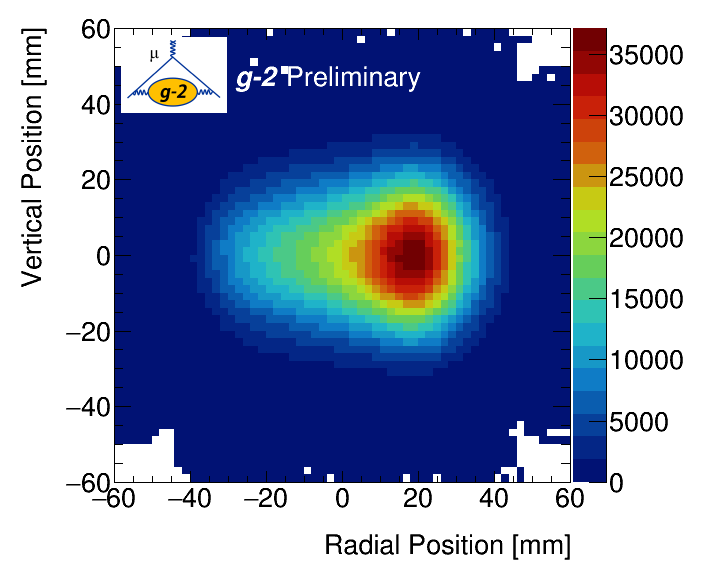
\includegraphics[width=0.7\textwidth]{BeamCrossSection}
    \caption[Extrapolated muon beam distribution cross-section]{Shown is a radial slice of the extrapolated muon distribution or beam spot.}
    \label{fig:BeamCrossSection}
\end{figure}



\begin{figure}[]
	\centering
	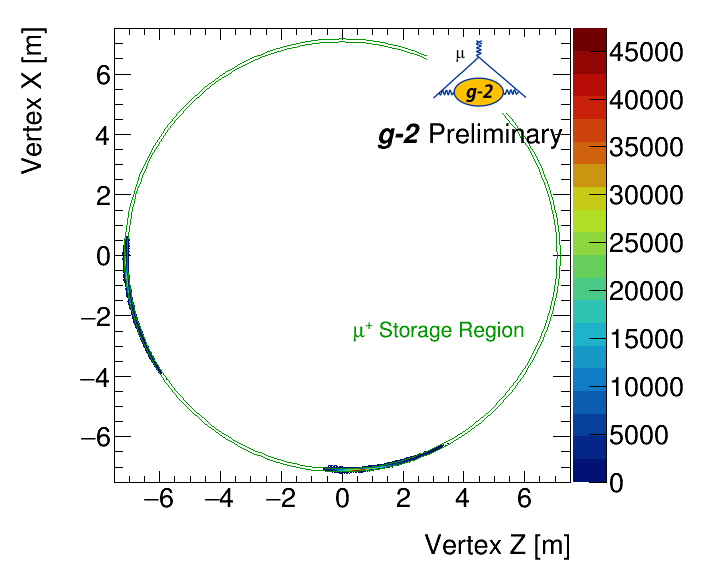
\includegraphics[width=0.9\textwidth]{VertexPlanView}
    \caption[Birds eye view of extrapolation in ring]{}    
    \label{fig:VertexPlanView}
\end{figure}




\cleardoublepage

%!TEX root = ../thesis.tex

\thispagestyle{myheadings}

\graphicspath{{Body/Figures/WaGeneral/Temporary/}{Body/Figures/WaGeneral/Reconstruction/}{Body/Figures/WaGeneral/Histogramming/}{Body/Figures/WaGeneral/Pileup/}{Body/Figures/WaGeneral/Pileup/TimeAndEnergySpectra/}{Body/Figures/RatioAnalysis/}{Body/Figures/RatioAnalysis/MethodOverview/}}

\chapter{\texorpdfstring{\wa}{wa} Measurement}
\label{chapter:wa}


The measurement of \wa is determined by counting the number of detected positrons in the calorimeters above some energy threshold, as described in \secref{section:WaIntro}. Doing so results in a histogram of counts which is modulated by \wa, \figref{fig:gm2wiggle}. Fitting for the frequency allows \wa to be extracted. The \wa measurement therefore consists of the steps needed to construct the histogram of counts, the fitting of that histogram, and any systematic studies done in the analysis. 


\section{Reconstruction of decay positron hits}
\label{sec:ReconWest}


The calorimeters measure hit times and energies of impacting particles, where these hit times and energies are determined from the raw SiPM signals and a reconstruction procedure. In E989 there are two overall separate reconstruction algorithms, \texttt{ReconWest} and \texttt{ReconEast}, both written in the \textit{art} framework similar to the tracking reconstruction. Each of these reconstruction algorithms is modularized, and the steps of the reconstruction process can be switched in and out at will. Using separate reconstruction methods gives confidence in any final results by removing single points of failure. The reconstruction method used in this analysis is \texttt{ReconWest}. A summary of its details will be presented here. A more thorough description is detailed by A. Fienberg \cite{AFThesis}.


The raw data are digitized waveforms, which are voltage versus time traces output from each SiPM for each calorimeter crystal hit. Due to the incredible amount of data coming in with the high muon fill rate, only those pulses which exceed some threshold are saved to disk. An online processing system checks the traces against this pre-configured threshold by passing all of the data through a GPU farm \cite{Gohn:2016shi}. If any trace is found above threshold, then the data is saved from every SiPM in every calorimeter, for a time range around the over-threshold trace. This time range is called a time island, similar to that in the tracking reconstruction, and typically has a width of $\SI{40}{ns}$ \cite{AFThesis}.


The traces are then fit with templates in order to extract the the area and peak times of any present pulses. Each SiPM has its own templates, one for positrons and one for laser pulses. These templates are extracted from data, where each template is determined by collecting many single pulse traces from a SiPM, normalizing by pulse area, aligning in time, and averaging them. These templates were checked against many systematic effects in order to make sure that the constructed templates did not bias the energy or time measurements, such as hit angle, energy (pulse size), position, and rate, as well as aging effects \cite{Kaspar:2016ofv,AFThesis}. Each trace is fit using a \chisq minimization algorithm with the corresponding SiPM templates in order to determine the time and energy of the hit. In order to fit for multiple pulses in a single time island, the fitting procedure first fits with a single template, and then checks the residuals for any remaining peaks. If peaks exist above some threshold, then the fitting is repeated until all pulses have been fit. The time measurement performance in the pulse finding was found to be unaffected by the number of pulses in a time island, and there is 100\% pileup separation at \ns{5} \cite{AFThesis}. See \figref{fig:TemplateFit} for a typical single template fit to a SiPM trace.


\begin{figure}[]
    \centering
    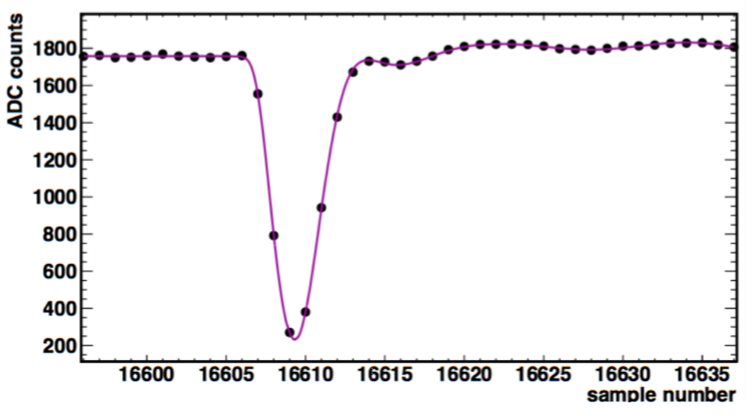
\includegraphics[width=0.6\textwidth]{TemplateFit}
    \caption[Template fit to SiPM trace]{A template fit in purple to a SiPM trace delineated by the black points which is in units of ADC counts. Plot courtesy of Aaron Fienberg.}
    \label{fig:TemplateFit}
\end{figure}


Once a pulse has been fit with a template, the pulse area needs to be converted to real energy units using an energy calibration procedure. A couple of different techniques exist that can be used, including a method that counts photo-statistics seen in the SiPMs \cite{AFThesis}. The default method used is a comparison of lost muon energy signatures in the calorimeters. As described in \refref{lostmuons}, muons lost from the storage ring can spiral inward and hit consecutive calorimeters with a specific time separation between calorimeter hits. These lost muons are minimum-ionizing particles, and thus leave a very distinct energy signature in the crystals, see \secref{sec:lostmuons}. Selecting on the time signature allows hits corresponding to lost muons to be isolated, and the energy signature can be used to determine the appropriate conversions from area to energy\footnote{Different channels can also be equalized based on the energy signatures.}. 


The energy calibration for positron hits as compared to lost muon hits then needs to be determined. Again there are a couple of different techniques, including a comparison of endpoint energies for high energy positrons which tail off at the magic momentum of $\SI{3.094}{\GeV}$, and comparison with simulation. The default technique is to calibrate the energies such that the optimal energy threshold for the \wa analysis is near $\SI{1.7}{\GeV}$ \cite{AFThesis}. Ultimately the energy calibration doesn't matter too much because it is not the energy units that really matter. What really matters is the number of positrons above some energy threshold, where that threshold can be optimized empirically. In fact, the entire \wa analysis could be done without even considering the energy of the incident positrons, and only considering the area of the SiPM pulses\footnote{This statement ignores the effects of pileup which must be accounted for, and applies for a threshold style analysis, and not for other analysis methods which depend on the energy of the pulses.}.


Each pulse fit now has an associated energy and time. Because the measurement of \wa depends heavily on the time reconstruction since the analysis is a frequency extraction, pulse times need to be corrected for various effects in order to reach the precision goal. The fitted times for each pulse need to be aligned on a fill-by-fill basis relative to the injection time of the beam, corrected for any channel differences due to differing pulse shapes or fiber lengths, and corrected for any calorimeter time misalignments due to the use of different laser system components. The fill-by-fill alignment is corrected for using the T0 detector as described in \secref{sec:T0}. The channel differences are corrected by aligning calorimeter channels in time using signals from islands with large simultaneous pulses in neighboring crystals. Calorimeters are time aligned using lost muon coincident events as described before. Once the times of the pulse fits or crystal hits have been determined, the energies can be corrected appropriately for gain effects measured by the laser system. As described in \secref{sub:LaserCalibrationSystem}, the laser calibration system corrects for in-fill, out-of-fill, and SDTP effects \cite{Gain}. \figref{fig:IFGFunction} shows an in-fill gain function fit to data for a single calorimeter. Systematic effects for corrected gain effects are studied in \secref{sub:gainerror}. 

\begin{figure}[]
    \centering
    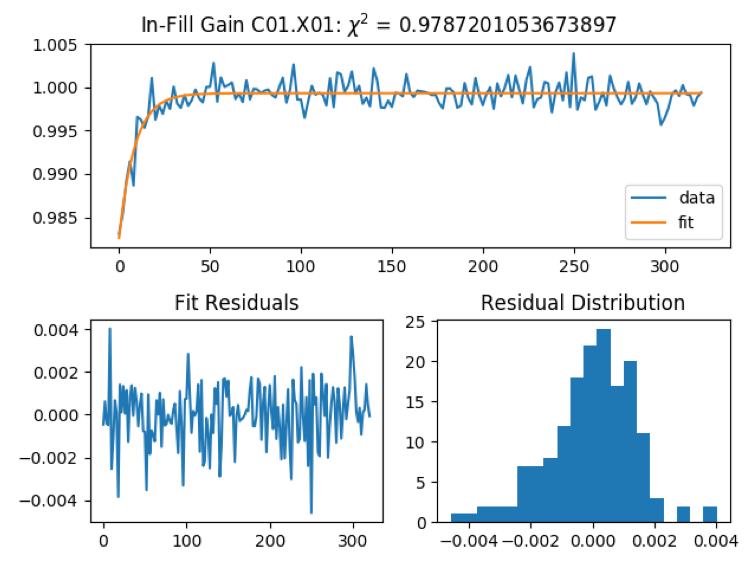
\includegraphics[width=0.6\textwidth]{IFGFunction}
    \caption[In-fill gain function fit for a single calorimeter crystal]{In-fill gain function fit for a single calorimeter crystal (top) and fit residuals (bottom). Each crystal has its own in-fill and SDTP gain function parameters. Plot courtesy of Matthias Smith.}
    \label{fig:IFGFunction}
\end{figure}


The last part of the calorimeter reconstruction is the clustering. Clustering is the stage which takes the individual template fit results from separate crystals, and turns them into the times, energies, and positions of decay positron impacts. For a time island with a single positron impact, the procedure is straightforward. The energy for the positron hit cluster is the sum of the individual hit crystal energies. The time for the cluster is taken as the time of the maximum energy hit in the island. This works because most of the deposited energy from a hit is localized to a single crystal. The position of the cluster is determined with a logarithmic weighting function between crystal hits, which for a $\SI{2}{\GeV}$ positron in the E989 calorimeters results in a resolution of $\SI{2}{mm}$ \cite{AFThesis}. See \figref{fig:CaloCluster} for a single calorimeter cluster from a positron hit in the calorimeter. For a time island with multiple positron impacts, the individual crystal hits are separated in time, where the time partitioning separates hits that are $\SI{2.5}{ns}$ apart, and the clustering proceeds as before. For hits which are within this time window, a pileup event has occurred. If the pileup event happens within the same crystal, then the multiple hits are measured as a single hit, and this needs to be corrected for using a pileup subtraction technique, as described in \secref{sub:pileupsubtraction}. For hits that occur in separate crystals, the pileup can be resolved using the spatial separation of the calorimeters. This is an ongoing area of work, and one technique is described in \refref{AFThesis}. For this analysis the spatial separation was turned off, which simplifies the analysis somewhat. This increases the amount of pileup seen in the data, which then needs to be handled by the pileup subtraction technique. For the precision of the Run 1 analysis result, this was found to be acceptable. 


\begin{figure}[]
    \centering
    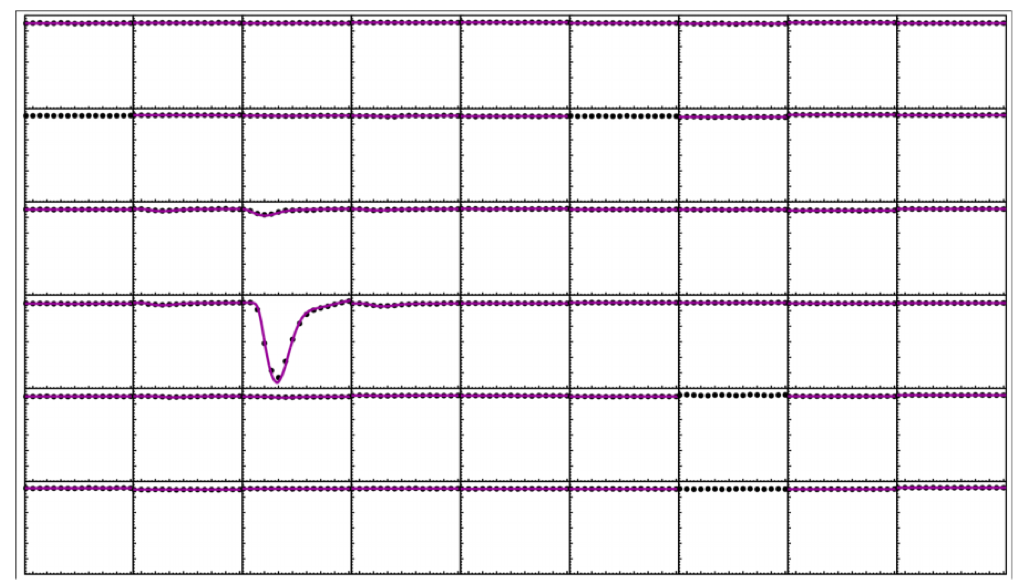
\includegraphics[width=0.9\textwidth]{CaloCluster}
    \caption[Calorimeter cluster from SiPM traces fit with templates]{A single positron hit in the calorimeter, which resulted in a reconstructed calorimeter cluster. Each box is a crystal in the calorimeter, where the contained trace is the SiPM output fit with a template. The positron hit the crystal three from the left and three from the bottom, where it deposited most of its energy. Some of the energy was deposited in the neighboring crystals. Plot courtesy of Aaron Fienberg.}
    \label{fig:CaloCluster}
\end{figure}



\section{Construction of hit energy and time spectra}
\label{sec:Histogramming}


Once the reconstruction has processed all calorimeter hits into clusters, the energy and time spectra histograms are made. At the very last stage of the reconstruction procedure, an \textit{art} module takes the produced clusters and puts them into \ROOT \texttt{TTree} formats, where individual data members include the energies, times, calorimeter numbers, etc. of the individual clusters. There is of order 20,000--140,000 cluster data files per dataset, which are combined down to order 200--1,400 \ROOT \texttt{TTree} files. These \ROOT \texttt{TTree}s are then passed through a \ROOT macro to produce \ROOT files with the histograms defined by the \texttt{TH1F} class, one \ROOT histogram file per tree file.


It should be noted that some of the parameter choices for the constructed histograms were informed by analysis results. All analysis parameters were chosen to be identical between the distinct analyzed datasets, in order to simplify both the comparison and combination of different dataset results. This section describes the justification for the different histogram parameters chosen. A table of the histogram parameters is shown in \tabref{tab:histogramparameters}.


\begin{table}[]
\centering
\setlength\tabcolsep{10pt}
\renewcommand{\arraystretch}{1.2}
\begin{tabular*}{.8\linewidth}{@{\extracolsep{\fill}}lc}
  \hline
    \multicolumn{2}{c}{\textbf{Time Spectra Parameters}} \\
  \hline\hline
    Parameter & Value \\
  \hline
    Energy threshold $(E_{th})$ & $\SI{1700}{\MeV}$ \\
    Bin width $(T_{c})$ & $\SI{149.2}{ns}$ \\
    Artifical dead time (ADT) & $\SI{6}{ns}$ \\
    Shadow dead time (SDT) & $\SI{6}{ns}$ \\
    Shadow gap time (SGT) & $\SI{12}{ns}$ \\
    Pileup energy scaling (C) & $1$ \\
    \gmtwo period $(T_{a})$ in Ratio Method & \mus{4.365411} \\
    Muon lifetime (\taumu) in Ratio Method & \mus{64.44} \\
  \hline 
\end{tabular*}
\caption[Parameters used in the construction of \wa time spectra]{Parameters used in the construction of \wa time spectra. \textbf{fill this table out more once I've gone through the various parts}}
\label{tab:histogramparameters}
\end{table}


Energy and time histograms are made for each individual calorimeter. These are summed together to form histograms of all hit times and energies. An energy threshold is applied to the clusters before filling the time histograms. As described at the end of \secref{section:WaIntro}, the optimal energy threshold is where the quantity $NA^{2}$ reaches the maximum, at least in the case of a five parameter fit\footnote{Using the final fit function and looking at the error directly on the fitted \wa frequency, a slightly better estimate can be found.}. By scanning over the choice of energy threshold and fitting the resulting time spectra with \equref{eq:5parfunc}, the optimal energy threshold can be determined as seen in \figref{fig:OptimalEnergyThreshold}. The optimal choice of energy threshold was determined to be $\SI{1700}{\MeV}$, in accordance with the cluster reconstruction energy calibration. 

    \begin{figure}[]
    \centering
        \begin{subfigure}[t]{0.45\textwidth}
            \centering
            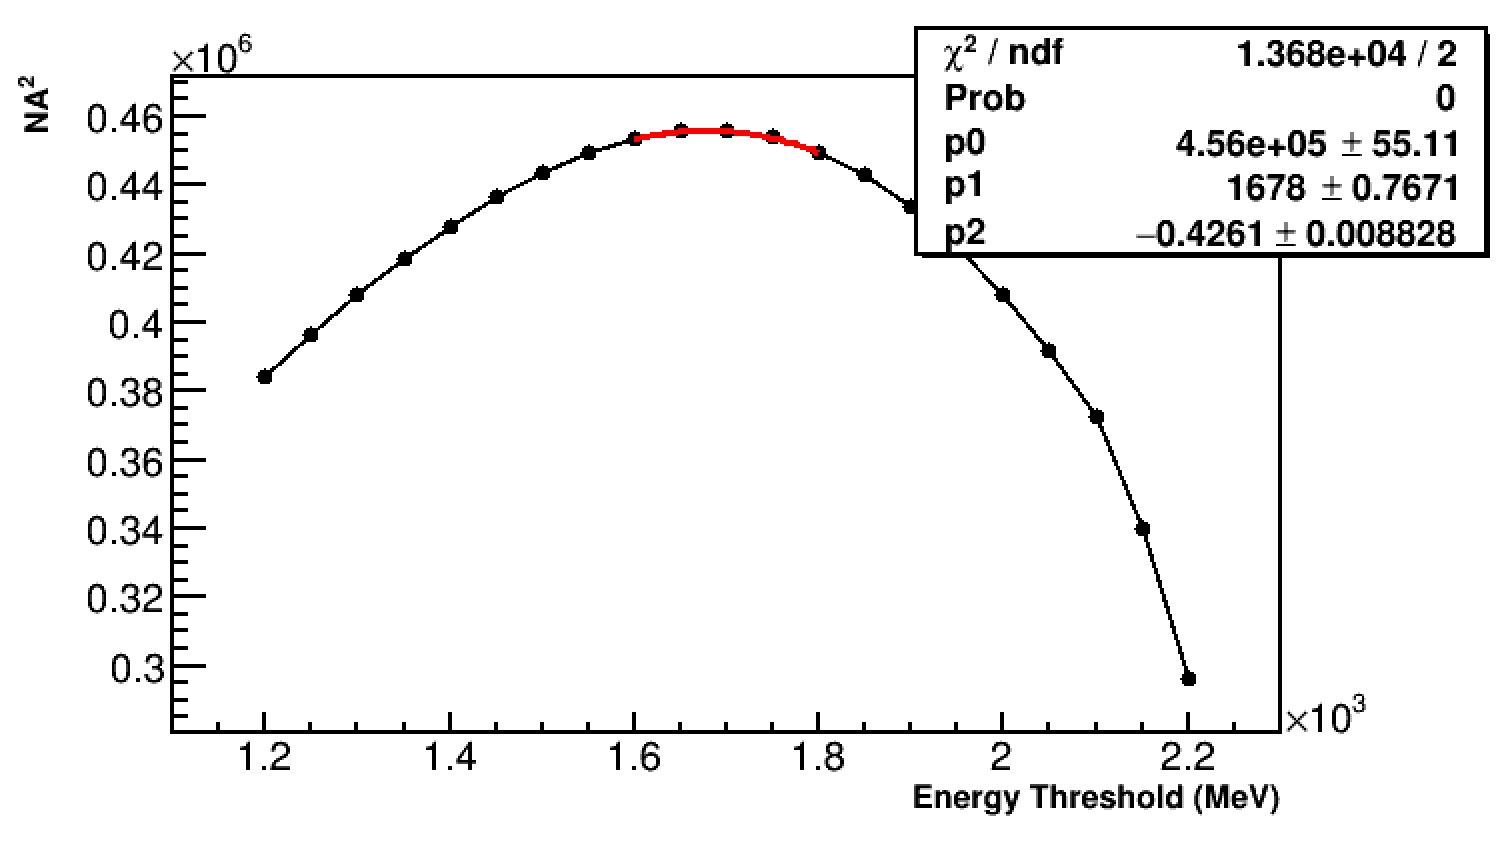
\includegraphics[width=\textwidth]{TemporaryEThresholdNA2}
            \caption{}
        \end{subfigure}
        \begin{subfigure}[t]{0.45\textwidth}
            \centering
            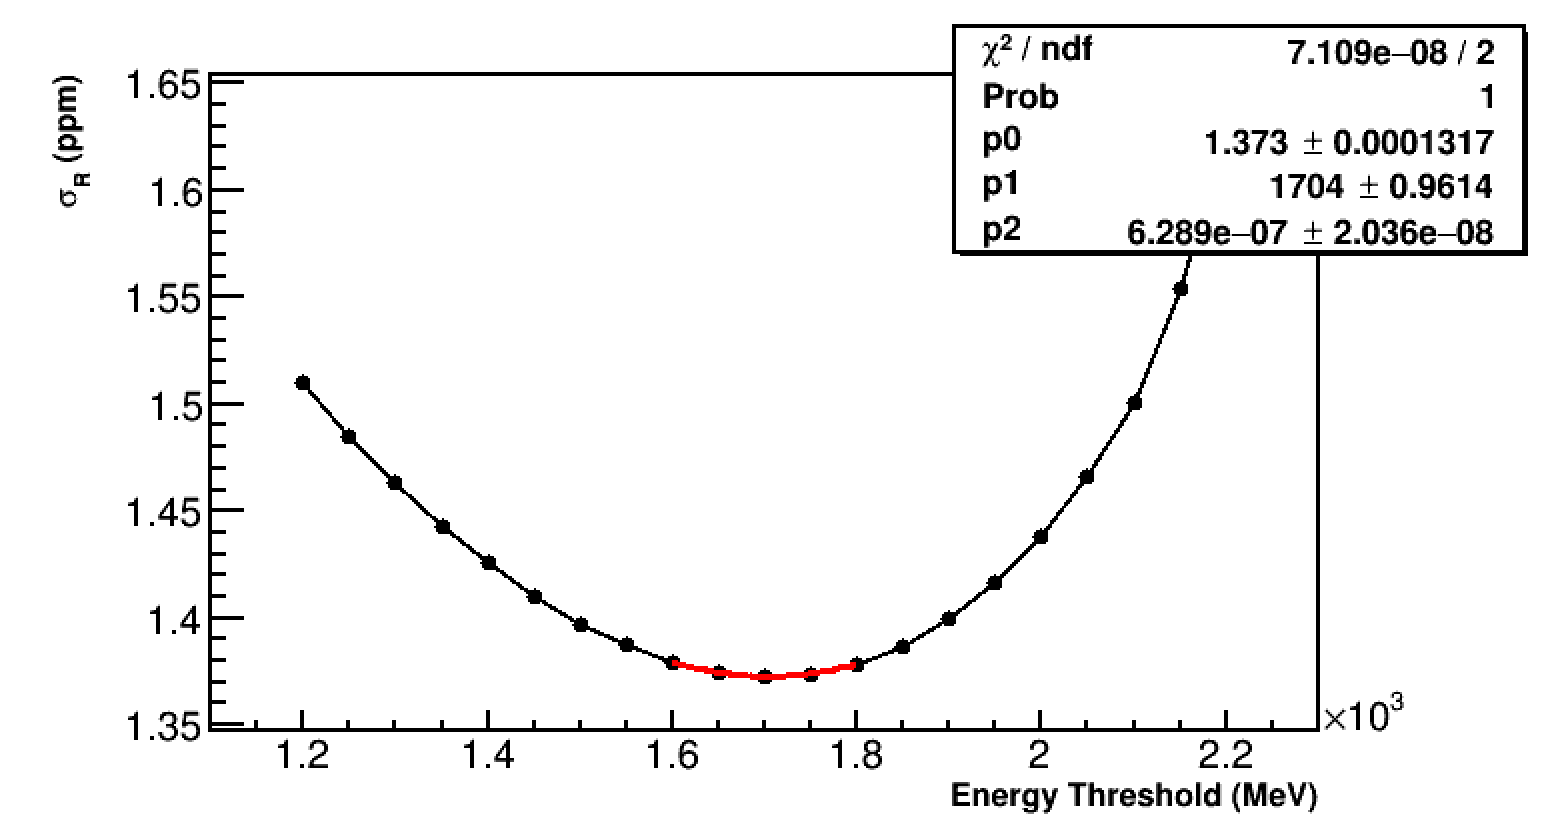
\includegraphics[width=\textwidth]{TemporaryEThresholdRatio}
            \caption{}
        \end{subfigure}% 
    \caption[Determination of optimal energy threshold]{The optimal energy threshold can be determined from the $NA^{2}$ quantity as described in \secref{section:WaIntro} from a five parameter fit to the data (left), or from the calculated error with the final fit function (right). \textbf{temporary energy threshold plots - replace - also not sure how to introduce R and ratio fit stuff here when I haven't talked about it yet}}
    \label{fig:OptimalEnergyThreshold}
    \end{figure}

% \begin{figure}[]
%     \centering
%     % \includegraphics[width=0.9\textwidth]{OptimalEnergyThreshold}
%     \rule{10cm}{10cm}
%     \caption[put caption here]{put a picture of the scanned optimal energy threshold here}
%     \label{fig:OptimalEnergyThreshold}
% \end{figure}


The optimal bin width for the time histograms was determined to be $\SI{149.2}{ns}$, the average of the cyclotron periods determined from a fast rotation analysis to the data \cite{fastrotationsomething}. As described in \secref{sub:beam_debunching}, this bin width combined with a time randomization on each cluster over a range of $\pm T_{c}/2 = \SI{149.2}{ns} / 2$ serves to eliminate the fast rotation signal in the data\footnote{Some analyzers randomize all times in a single fill by half the cyclotron period as opposed to each individual pulse.}. This randomization is done using \ROOT's \texttt{TRandom3} class. The default random seed for each histogram \ROOT file is the hash of the input file name using C++'s standard hash class. Histograms are defined with a time range of 0--\mus{699.8972} (the closest integer multiple of the bin width to \mus{700}), corresponding to 4691 bins. Clusters with times $<$ \mus{25} or $>$ \mus{660} are dropped, corresponding to 4256 bins containing data.




-include sam dataset names here or in the run 1 section?
-I should probably talk a little bit about the energy spectra as well
- need to mention how the spectra are split into different calorimeters
-should I show an energy spectra here without the pileup subtracted - I need to talk about the lost muon peak 


\subsection{Pileup subtraction}
\label{sub:pileupsubtraction}


As described in \secref{sec:Calorimeters}, there will be a certain amount of pileup in the detectors. Pileup again is the term for when multiple particles hit a calorimeter within the dead time of the detector such that they are registered as a single hit or cluster. The measured energy and time spectra for all observed clusters will include this pileup background. For the energy threshold time histogram, the number of counts will be wrong for cases where two below-threshold particles are registered as a single cluster above threshold, and where two above-energy threshold particles are registered as a single cluster. In the former, an extra count is added into the histogram, and in the latter a count is missed. The case where two lower energy positrons are registered as a single higher energy cluster will have a different \gmtwo phase than an actual single cluster at the same energy. This is because the lower energy positrons on average decay from muons which have travelled further around the ring, due to acceptance effects. These muons which have travelled further around the ring have spent more time in the magnetic field, and thus their spins have precessed more. See \figref{fig:PileupExample}. Clusters which originate from pileup events therefore have a different \gmtwo phase than non-pileup events. 


If pileup was a constant effect, then the phase of the time histogram would be shifted by some constant amount, and the extracted \wa frequency would be unaffected. However, the rate of pileup in the detectors changes over the time of a fill, as muons decay away. The rate of double pileup events in the detectors, where the word double indicates cases where two hits are registered as a single cluster, will go approximately as half the rate of single hit events\footnote{It is not exact when including the non-linear dead time of the detectors}, and similarly for triple and higher orders of the pileup effect. Because the rate of hits in the detectors oscillates at the \gmtwo frequency, pileup will increase and decrease accordingly leading to oscillations in the pileup time spectra at \wa and 2\wa. The lifetime of the overall pileup effect is approximately half the lifetime at which clusters are registered in the detectors, at \taumu, since double pileup is the dominant contribution. In order to to extract the correct \wa frequency, the pileup effect thus needs to be included in the fit function or subtracted out of the data. The former is challenging due to the non-linear nature of the dead time of the detectors, and would in the end include another phase in the argument of the cosine term in the fit function, thus worsening the statistical precision of the extracted \wa frequency. All analyzers thus construct an approximation of the pileup effect and subtract it from the data before fitting.


% -need to mention the \% level effect of pileup - ~1\% but where do you get that number...


\begin{figure}[]
    \centering
    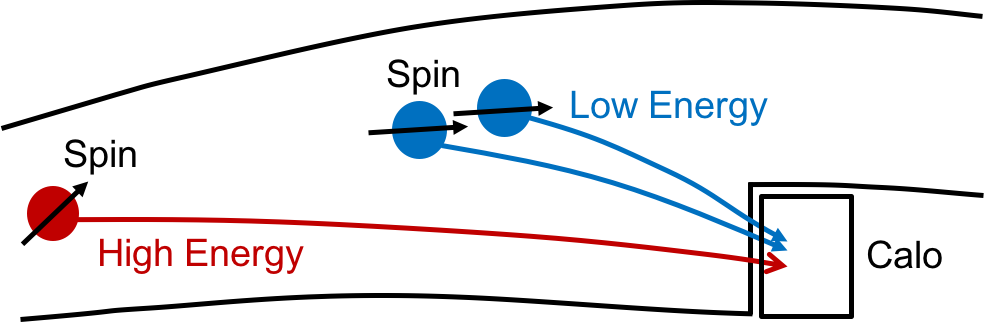
\includegraphics[width=0.5\textwidth]{PileupExample}
    \caption[Pileup example]{Pileup example, where two low energy positrons are registered as a single high energy positron. The black arrows indicate the (exaggerated) direction of the muon spins at the time of decay. Because of acceptance effects the lower energy decay positrons typically come from muons which have traveled further around the ring, and thus the muon spins have precessed more in the magnetic field, leading to a different measured \gmtwo phase for pileup events.}
    \label{fig:PileupExample}
\end{figure}


There are various methods to construct pileup spectra which are then subtracted off the main time and energy spectra. The method used in this analysis is called the `asymmetric shadow method', originally developed in E821 \cite{E821PileupShadow}. This method statistically constructs an approximation for the pileup from the data by assuming that the probability of observing a pileup pulse is the same as the probabilty that two pulses will be offset by some small amount of time, such as \ns{10}. The method works by looking in time windows after trigger pulses to see if a `shadow' pulse exists. If such a pulse exists, then a shadow doublet is created, see \figref{fig:ShadowPileupMethod}. The width of the time window, and the time offset from the trigger pulse to the window, are called the shadow dead time (SDT) and shadow gap time (SGT) respectively. The times and energies of the constructed pileup doublets are taken as
            \begin{gather}
                E_{\text{doublet}} = C \cdot (E_{1} + E_{2}), \label{eq:Edoublet} \\
                t_{\text{doublet}} = \frac{t_{1} \cdot E_{1} + (t_{2}-SGT) \cdot E_{2}}{E_{1} + E_{2}}, \label{eq:tdoublet}
            \end{gather}
where the energy of the doublet is the sum of the two singlet pulses $E_{1,2}$ times some calibration constant $C$, with a default value of 1, and the time of the doublet is the energy-weighted time of the two singlets $t_{1,2}$. The procedure for constructing the pileup spectra is as follows:
\begin{itemize}
    \item{Put each hit into a vector corresponding to a specific fill and a specific calorimeter}
    \item{Time order the hits}
    \item{Loop through the hits, for each hit look within a window of width SDT a time SGT later to see if a shadow pulse exists}
    \item{If a shadow pulse exists, construct a shadow doublet with energies and times as defined in Equations~\ref{eq:Edoublet} and \ref{eq:tdoublet}}
    \item{Randomize $t_{\text{doublet}}$ over the range $\pm T_{c}/2$ (to remove fast rotation as before, \secref{sub:beam_debunching})}
    \item{Per calorimeter, construct pileup energy and time spectra as $P = D - S$, where $D$ is the sum of doublets and $S$ is the sum of singlets used in the construction of the doublets, with the times of the singlets set as $t_{\text{doublet}}$; when constructing the pileup time spectra, only include those doublets and singlets above the energy threshold}
\end{itemize}
Thus pileup energy and time spectra are constructed for each calorimeter, which can then be subtracted off the calorimeter cluster energy and time histograms. When combining the data, the individual pileup histograms are simply added together before subtraction off the calorimeter sum histograms. 


In order to produce an estimate of the pileup spectra which best matches the data, an artifical dead time (ADT) is applied to the data before time randomization. This is done because the true dead time of the detectors depends on the energies and spatial separation of the incoming hits. While this is a small effect, by applying an artificial deadtime and matching the shadow window time, the pileup estimation is improved slightly. The construction of the artificial pileup is handled in the same way as the construction of the shadow pileup, with SGT set to \ns{0}. The constructed artificial doublets replace the singlets in the data. The value for the ADT and SDT is set at \ns{5}, the time threshold at which pileup is 100\% resolved. 

The value of the SGT is simply set to twice the SDT, in order to push the shadow window out to times well beyond the dead time of any pileup events, but not so far that an appreciable fraction of muons have decayed. The value of the doublet energy scaling factor C is set to 1, which is a fine approximation as the spatial separation in the reconstruction is turned off\footnote{With the spatial separation turned off, `pileup' events can occur in crystals that are easily separated by eye. While this increases the level of pileup seen in the data, the pileup approximation method also does not consider the spatial separation, and thus handles the level of pileup accordingly.}. The values for each pileup parameter is shown in \tabref{tab:histogramparameters}. See \secref{sub:pileuperror} for systematic studies on the effect on \wa due to these chosen parameters.



\begin{figure}[]
    \centering
    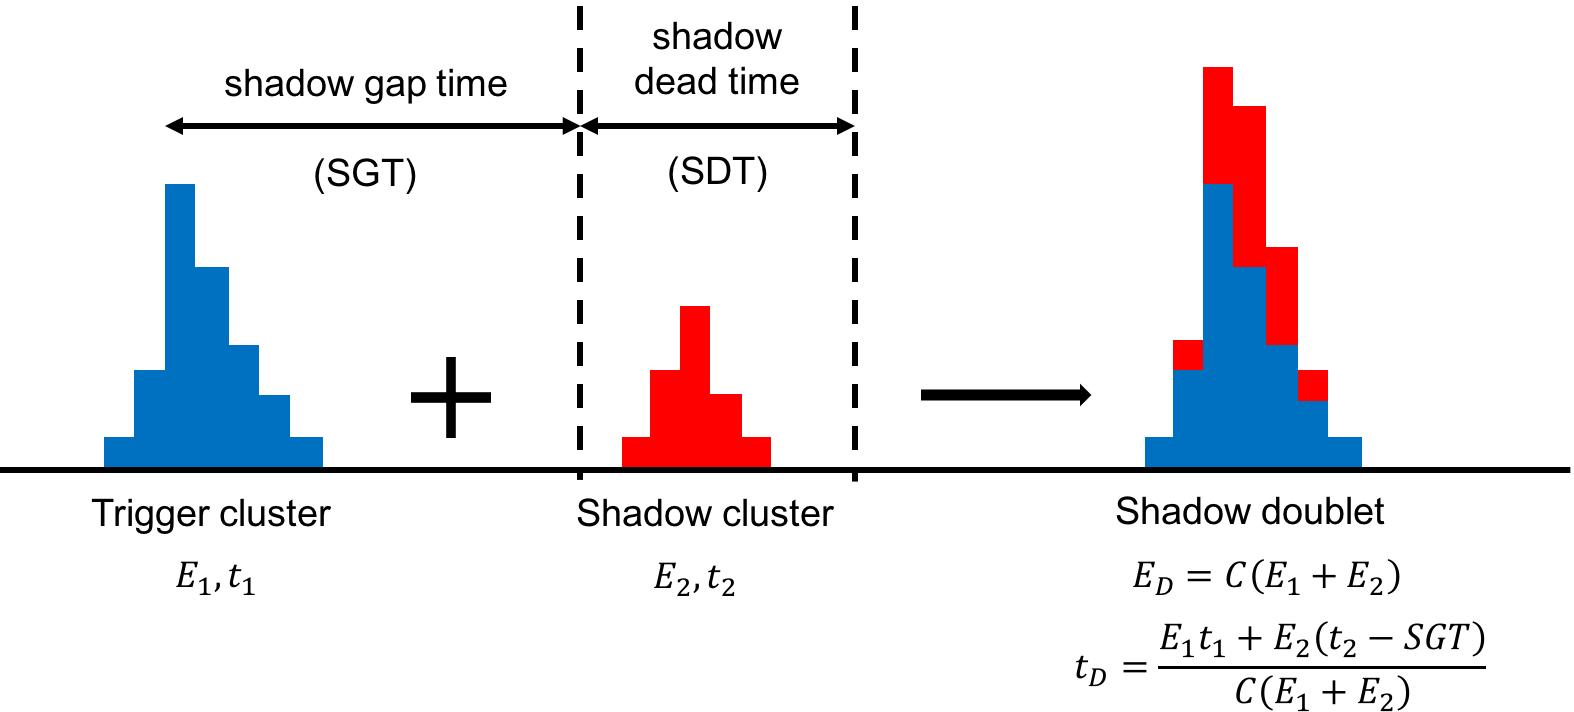
\includegraphics[width=\textwidth]{ShadowPileupMethod}
    \caption[Shadow pileup method]{}
    \label{fig:ShadowPileupMethod}
\end{figure}


The pileup energy spectra as compared to the cluster energy spectra is shown in \figref{fig:ClusterEnergiesVsPileupEnergies}. In general, the two lobes starting at approximately $\SI{3}{\GeV}$ and $\SI{6}{\GeV}$ consist of double and triple pileup events respectively\footnote{All orders of pileup fill out the whole energy range, but certain areas consist of mostly one or the other.}. It can be seen that the shadow method of pileup construction produces a pileup energy spectra which is a decent approximation of the cluster energies above the maximum energy that a single decay positron would have at $(\SI{3.094}{\GeV}) + \text{detector resolution}$, for cases of double and even triple pileup. The shape difference arises from two factors: First, the shadow method is only written to construct doublets, and does not consider cases of triple or higher orders of pileup. Second, the real pileup in the data contaminates the construction of the shadow pileup spectra, such that a shadow doublet can be constructed from real pileup pulses. While this alleviates the triplet problem slightly, it means that the doublet pileup spectrum is slightly wrong. The corrected energy spectra (cluster energies minus pileup energies), can be seen in \figref{fig:AddedEnergies}. The shape mismatch is even more apparent as the corrected energy spectrum is high for energies above the expected tail of the true energy distribution, and then goes negative before tailing off to zero. It has been determined that regardless of this shape mismatch, the systematic error on the extracted \wa frequency due to the pileup is within the target uncertainty for the level of statistics in the Run~1 dataset, \secref{sub:pileuperror}. This is in part due to the fact that it is the pileup time spectrum that is most important, as opposed to the pileup energy spectrum. The pileup time spectrum for those pileup pulses above energy threshold is shown in \figref{fig:PileupTimeSpectrum}. Finally, since the pileup is statistically constructed and then subtracted from the data, the errors on the final time histogram are no longer Gaussian. The proper calculation of the errors is detailed in \appref{app:PileupErrors}.


    \begin{figure}[]
        \centering
        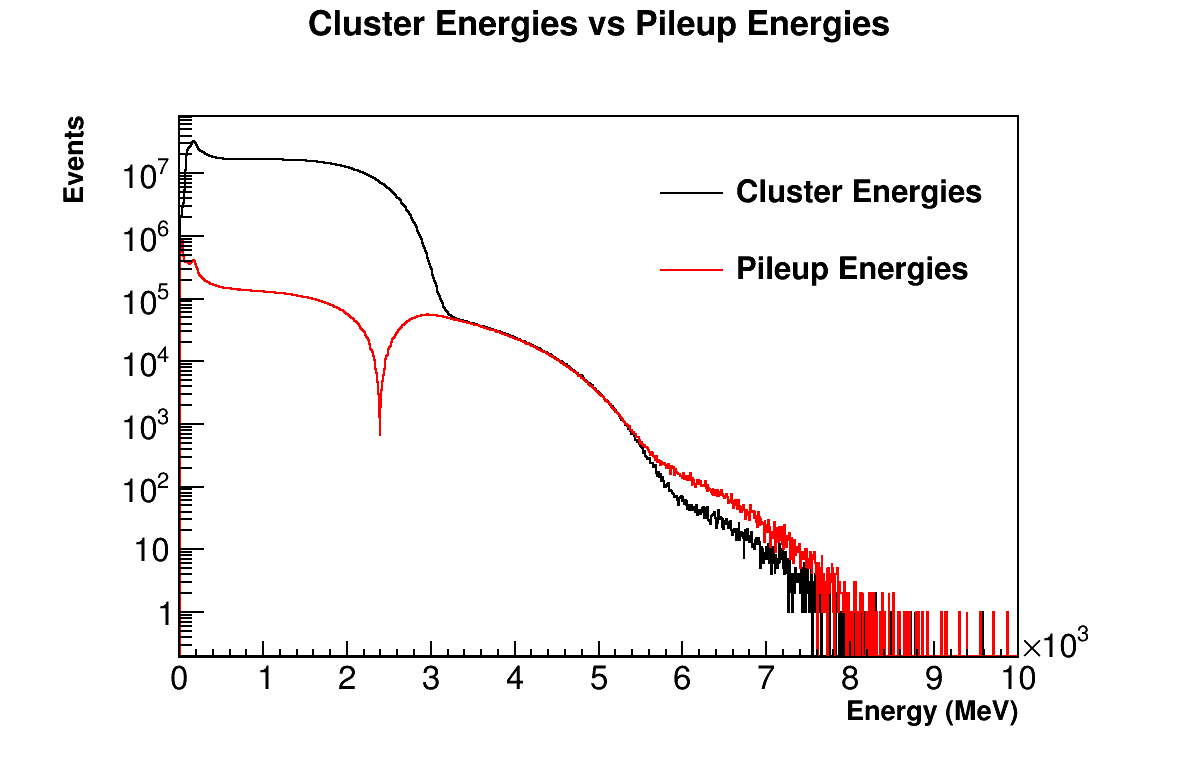
\includegraphics[width=\textwidth]{ClusterEnergiesVsPileupEnergies}
        \caption[Cluster energies vs pileup energies]{Cluster energies in black are plotted vs pileup energies in red, for all calorimeters added together, plotted on a log scale. At energies below about 2.4 GeV the pileup energy spectrum goes negative. In this plot the absolute value of the pileup energies is plotted, and a spike at about 2.4 GeV can be seen as a consequence of this. The shapes do not match perfectly for the constructed pileup spectra, which can be seen at high energies. It should be noted that for energies above $\SI{3.094}{\GeV}$ there is still a shape mis-match even though the red and black curves overlap due to the plotting scale.\textbf{update pictures with latest data, improved captions, and plotting styles}}    
        \label{fig:ClusterEnergiesVsPileupEnergies}
    \end{figure}


    \begin{figure}[]
    \centering
        \begin{subfigure}[]{0.8\textwidth}
            \centering
            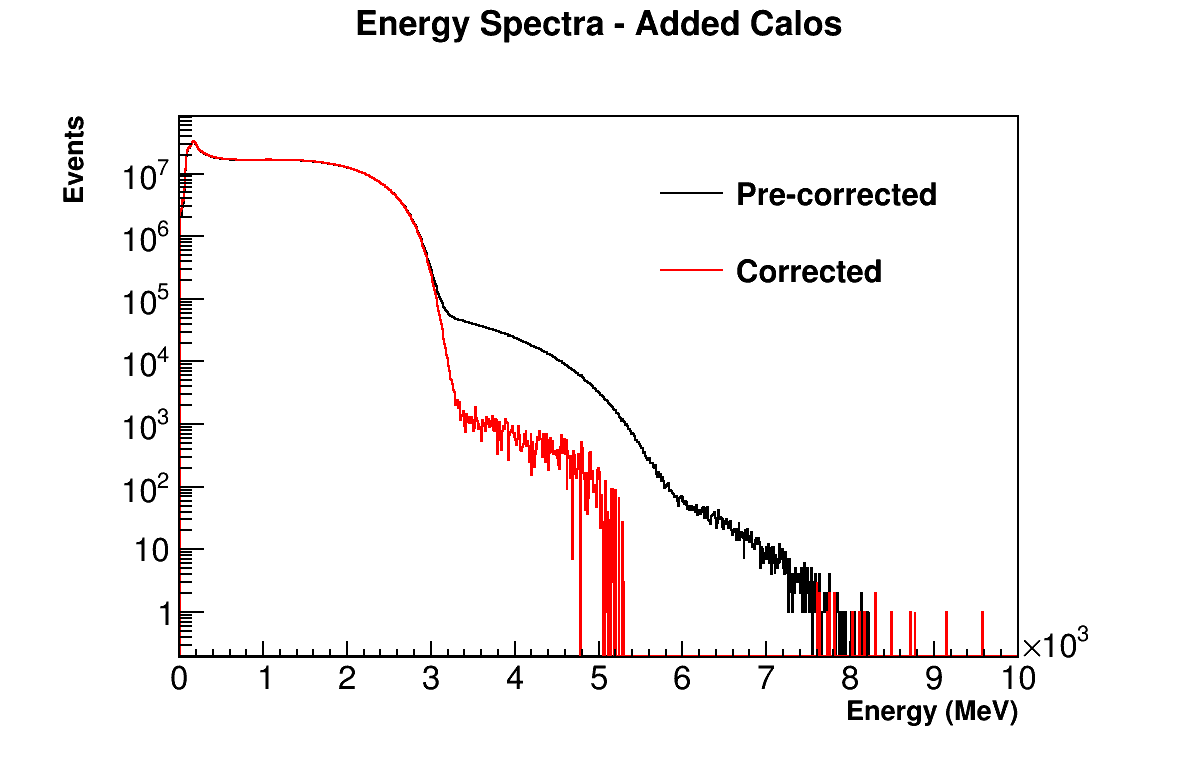
\includegraphics[width=\textwidth]{AddedEnergies}
            \caption{Log scale - the corrected energy spectrum goes negative around 5 GeV.}
        \end{subfigure}% %you need this % here to add spacing between subfigures
        \vspace{1cm}
        \begin{subfigure}[]{0.8\textwidth}
            \centering
            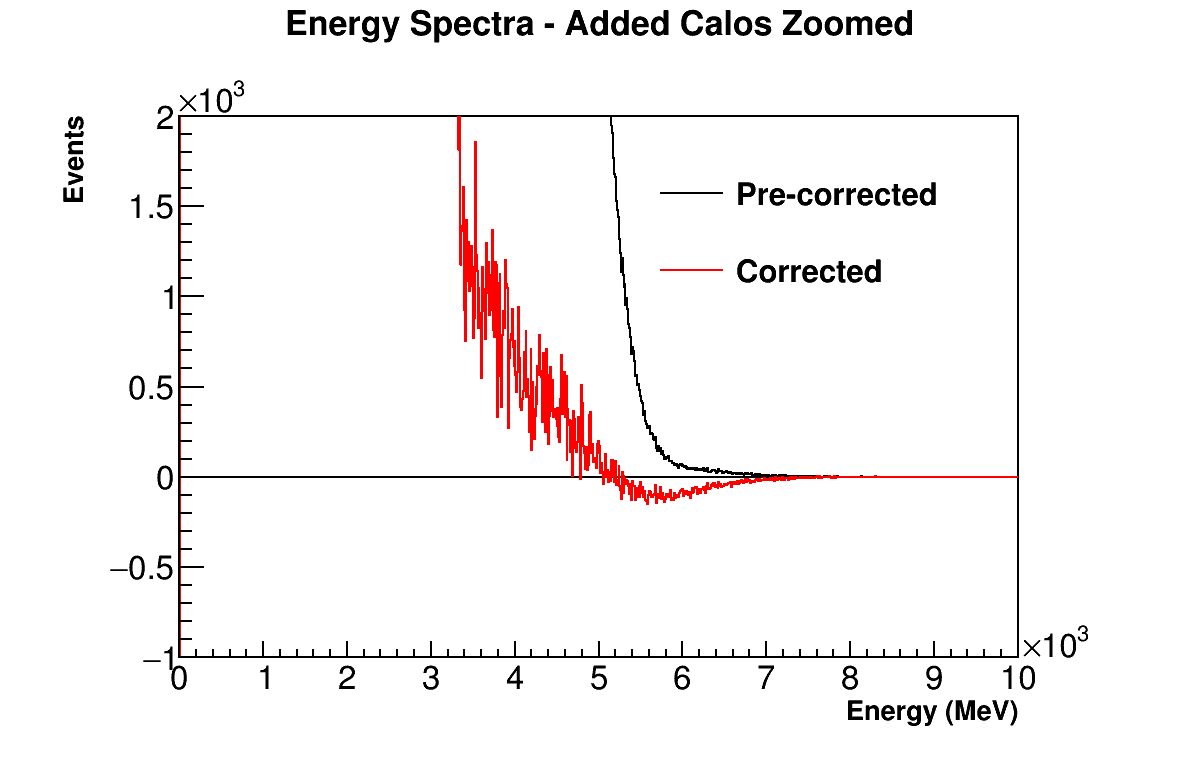
\includegraphics[width=\textwidth]{AddedEnergiesZoomed}
            \caption{Linear scale - zoomed in to show the shape.}
        \end{subfigure}
    \caption[Non-corrected and pileup corrected cluster energies]{Plots for the pre-corrected and corrected energy spectra are shown, all calorimeters added together. Because the triplets and contamination are not accounted for, the corrected energy spectrum does not lie exactly along zero above the energy response of the detectors.\textbf{update pictures with latest data, improved captions, and plotting styles}}
    \label{fig:AddedEnergies}
    \end{figure}


    \begin{figure}[]
        \centering
        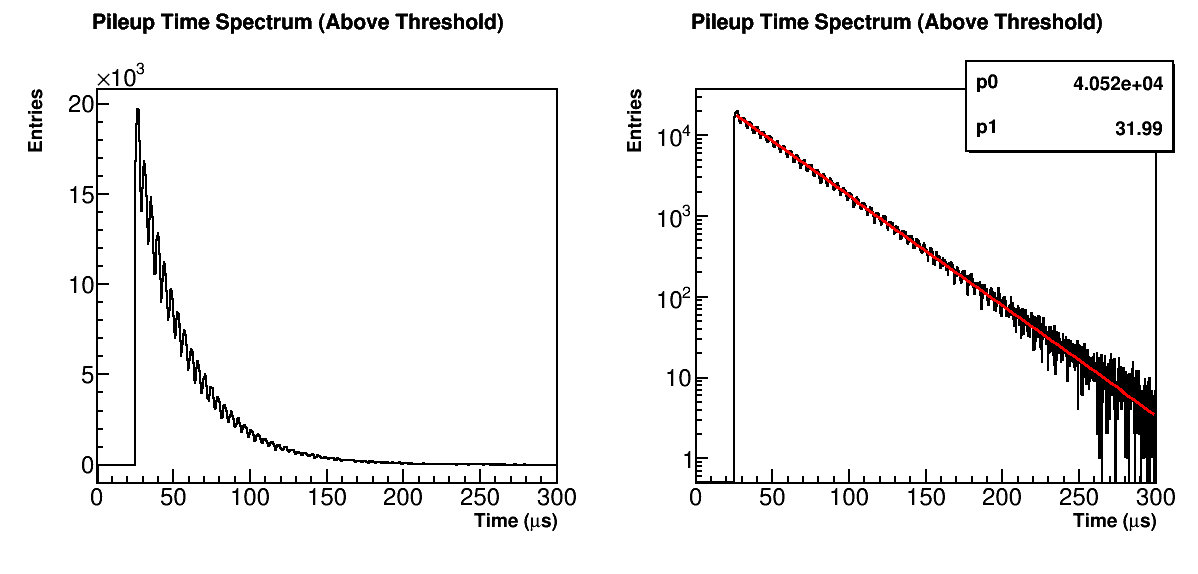
\includegraphics[width=\textwidth]{PileupTimeSpectrum}
        \caption[Pileup time spectrum above threshold]{Plotted is constructed pileup time spectrum on a linear (left) and log (right) scale. The histogram on the right is fit to a simple two parameter exponential to get an idea of the lifetime of the pileup, calculated here as $\SI{31.99}{\mu s}$, which is close to half of the muon lifetime at about $\SI{64.44}{\mu s}$.\textbf{update pictures with latest data, improved captions, and plotting styles}}
        \label{fig:PileupTimeSpectrum}
    \end{figure}





-should I show per calorimeter pileup energy and time spectra????



    % \begin{figure}[]
    %     \centering
    %     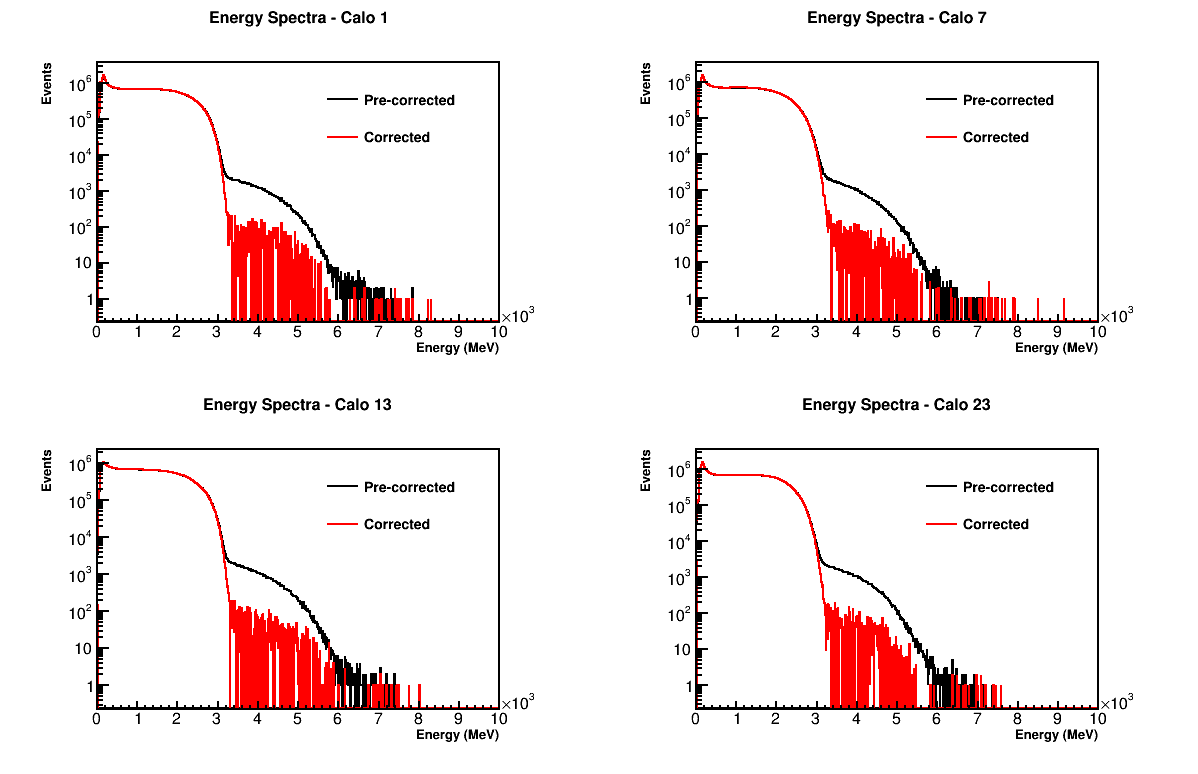
\includegraphics[width=.8\textwidth]{CaloEnergies}
    %     \caption[CaloEnergies]{Pre-corrected and corrected energy spectra for calorimeters 1, 7, 13, and 23 plotted on a log scale.}    
    %     \label{fig:CaloEnergies}
    % \end{figure}

    % \begin{figure}[]
    %     \centering
    %     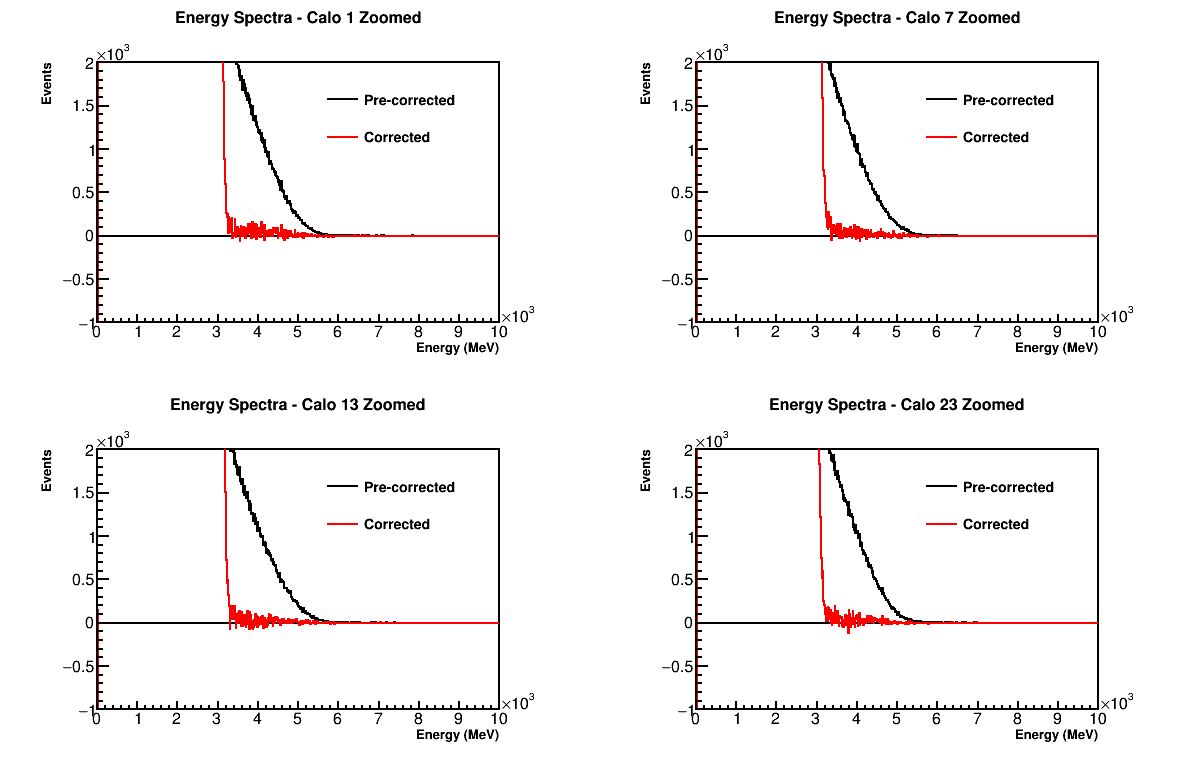
\includegraphics[width=.8\textwidth]{CaloEnergiesZoomed}
    %     \caption[CaloEnergiesZoomed]{Pre-corrected and corrected energy spectra for calorimeters 1, 7, 13, and 23 plotted on a linear scale and zoomed in.}    
    %     \label{fig:CaloEnergiesZoomed}
    % \end{figure}




% https://gm2-docdb.fnal.gov/cgi-bin/private/RetrieveFile?docid=13963&filename=PileupScaleShadowTesting.pdf&version=1
% https://gm2-docdb.fnal.gov/cgi-bin/private/RetrieveFile?docid=14394&filename=PileupFormEtc.pdf&version=2




\subsection{Ratio Method}


The method used in this analysis to extract \wa is called the ``Ratio Method.'' It is a technique that modifies the data in such a way that the exponential decay in the time histogram is removed, and slow effects are reduced. It was used successfully in the E821 experiment \cite{JKThesis,LDThesis,JPThesis}. The method works by dividing the data into four separate datasets, one with the times of all clusters shifted up by half a \gmtwo period, $+$\Tatwo, one with times shifted down by half a \gmtwo period, $-$\Tatwo, and two left alone. Assuming the data is described by the five parameter function \equref{eq:5parfunc} shown in \figref{fig:fiveparamfunc} (repeat it here?), and that the data is equally split into four, then the new four datasets are given as:
    \begin{equation}
    \begin{aligned}
        u_{+}(t) &= \frac{1}{4} N_{5}(t+T/2) \\
        u_{-}(t) &= \frac{1}{4} N_{5}(t-T/2) \\
        v_{1}(t) &= \frac{1}{4} N_{5}(t) \\
        v_{2}(t) &= \frac{1}{4} N_{5}(t)
    \end{aligned}
    \end{equation}
To be explicit here regarding the signs, the counts that are filled into the histogram described by $u_{+}$ have their times shifted as $t \rightarrow t - T/2$, which is what the function $N_{5}(t+T/2)$ describes, and vice versa for $u_{-}$. In order to time shift the data as such, \Ta needs to be known a priori to high precision. The value used is taken from the E821 result, and its value is taken as $1/f_{a}$, where $f_{a}$ is \SI{0.2290735}{MHz}:
        \begin{align}
            T_{a} \approx \SI{4.365411}{\mu s}
        \label{eq:Ta}
        \end{align}
This value for $f_{a}$ was determined by averaging column 2 of Table XV of the E821 Final Report \cite{E821FinalReport}, which consits of the $f_{a}$ results for the different run periods in that experiment. A systematic error on the choice of this parameter is calculated in \secref{sub:gm2periodGuess}.


The datasets are then combined as 


-show u and v here and point to figures...





-detail the ratio method - might need to pull stuff out from my appendix 

-referance taumu and Ta and point to table 

-perhaps cite redin statistics paper again for weighting scheme


-A full derivation is given in appendix...


    \begin{figure}[]
    \centering
        \begin{subfigure}[t]{0.45\textwidth}
            \centering
            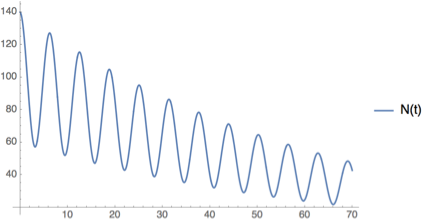
\includegraphics[width=\textwidth]{FiveParamFunc}
            \caption{}
        \label{fig:fiveparamfunc}
        \end{subfigure}%

        \vspace{2mm}
        \begin{subfigure}[t]{0.45\textwidth}
            \centering
            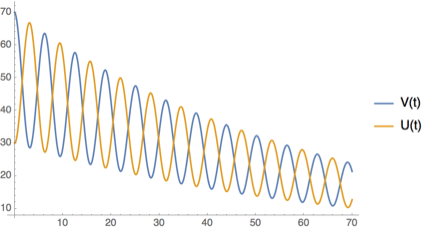
\includegraphics[width=\textwidth]{UVFuncs}
            \caption{}
        \label{fig:UVfuncs}
        \end{subfigure}
        \begin{subfigure}[t]{0.45\textwidth}
            \centering
            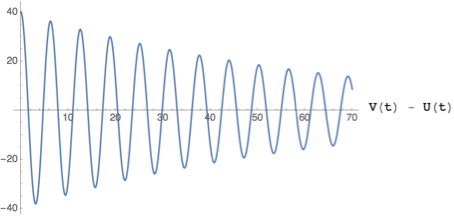
\includegraphics[width=\textwidth]{RatioNumFunc}
            \caption{}
        \label{fig:rationumfunc}
        \end{subfigure}%
        \vspace{2mm}
        \begin{subfigure}[t]{0.45\textwidth}
            \centering
            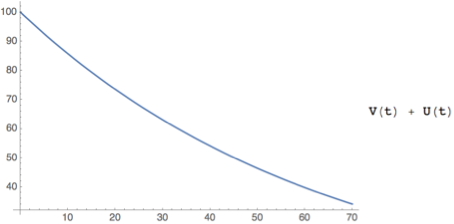
\includegraphics[width=\textwidth]{RatioDenomFunc}
            \caption{}
        \label{fig:ratiodenomfunc}
        \end{subfigure}
        \begin{subfigure}[t]{0.45\textwidth}
            \centering
            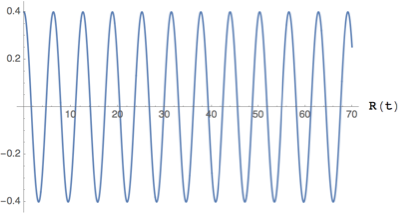
\includegraphics[width=\textwidth]{RatioFunc}
            \caption{}
        \label{fig:ratiofunc}
        \end{subfigure}% 
    \caption[]{\textbf{should I just use the ones I make with the data or no?}}
    \label{}
    \end{figure}



-mention how I create 4 pileup histograms for the ratio ...






\section{Lost muons}
\label{sec:lostmuons}

-need to include delta t plot and energy deposition plot
-this should potentially be in the fitting section...


\cite{lostmuons}




\section{Fitting}
\label{sec:Fitting}


-should I include stuff about my tmethod fits? just basic fit results but no systematic studies and all that?
-a root macro is used to fit the data, and then to make plots


Fit is from \mus{30.2}--\mus{650}, corresponding to 4154 bins.


\begin{table}[]
\centering
\setlength\tabcolsep{10pt}
\renewcommand{\arraystretch}{1.2}
\begin{tabular*}{.8\linewidth}{@{\extracolsep{\fill}}lc}
  \hline
    \multicolumn{2}{c}{\textbf{Fit Procedure Parameters}} \\
  \hline\hline
    Parameter & Value \\
  \hline
    Fit start time & \mus{30.2} \\
    Fit end time & \mus{650} \\
  \hline 
\end{tabular*}
\caption[]{\textbf{fill this table out more once I've gone through the various parts}}
\label{tab:fitprocedureparameters}
\end{table}






\subsection{CBO terms}
\label{sub:cboterms}






\section{Systematic errors}
\label{sec:Systematic Errors}



\begin{table}[]
\centering
\setlength\tabcolsep{10pt}
\renewcommand{\arraystretch}{1.2}
\begin{tabular*}{.8\linewidth}{@{\extracolsep{\fill}}lc}
  \hline
    \multicolumn{2}{c}{\textbf{\wa Measurement Uncertainties}} \\
  \hline\hline
    Source of uncertainty & E989 Goal (ppb) \\
  \hline
    Gain changes & 20 \\
    Pileup & 40 \\
    Lost muons & 20 \\
    CBO & 30 \\
    E field and pitch corrections & 30 \\
  \hline
    Quadrature sum & 70 \\
  \hline 
\end{tabular*}
\caption[Uncertainties in the precession frequency measurement]{Systematic errors in the precession frequency measurement. \textbf{fill this table out more once I've gone through the various parts}}
\label{tab:wauncertainties}
\end{table}




\subsection{Gain}
\label{sub:gainerror}


-talk about the equations here - slight reference to either detector section or reconstruction section in this chapter



\subsection{Pileup}
\label{sub:pileuperror}


For errors relating to the choice of SDT and SGT - the idea is this: Show the plots which show how the choices of SDT and SGT don't matter as long as the automatic pileup scaling is applied (shapes are the same) - this implies that the error due to these guys is contained within the pileup multiplier error, and can thus be ignored in favor of the latter - point back to pileup section when talking about this - I can also potentially if I have time do scans on these parameters and look at the effect on R

% https://gm2-docdb.fnal.gov/cgi-bin/private/RetrieveFile?docid=13963&filename=PileupScaleShadowTesting.pdf&version=1
% https://gm2-docdb.fnal.gov/cgi-bin/private/RetrieveFile?docid=14394&filename=PileupFormEtc.pdf&version=2


-pileup multiplier - amplitude
-pileup time shift - phase
-pileup energy scaling - phase



\subsection{gm2 period guess}
\label{sub:gm2periodGuess}


\cleardoublepage

\cleardoublepage

%!TEX root = ../thesis.tex

\thispagestyle{myheadings} % should I be including this at the top of every section page??

\chapter{Conclusion}
\label{chapter:Conclusion}


Experiment E821 measured the anomalous magnetic moment of the muon to a relative uncertainty of 540 parts per billion, corresponding to a discrepancy of three to four standard deviations from the Standard Model theoretical value. In order to confirm or deny this discrepancy, a new experiment has been undertaken to measure the same quantity. E989 measures \amu by measuring the spin precession frequency of muons within a magnetic storage ring and the strength of the magnetic field within the storage region. The former is done by counting the number of decay positrons observed in electromagnetic calorimeters above an energy threshold, while the latter is done using NMR probes in and around the muon storage region. 



Straw trackers assist both measurements by measuring muon beam dynamics which directly impact both the precession frequency measurement and the distribution of muons within the measured magnetic field. In \chapref{chapter:TrackReconstruction} this dissertation presented the track fitting algorithm used in the reconstruction of decay positron tracks necessary for reconstructing muon beam decay vertices. The track fitting method, Geane, propagates positrons in the full E989 Geant4 simulation with the advantage of direct access to the geometry, material, and non-uniform magnetic field present within the tracker region. Transport matrices, error matrices, and predicted parameter vectors are generated which are then used in a global \chisq minimization algorithm which produces an optimal state vector at the entrance to the tracker. This state vector is then extrapolated back into the storage region to approximate muon decay points, from which the muon distribution and beam motion can be derived. The coherent beam motion has been well characterized both radially and vertically. Radially, the beam is seen to oscillate inwards and outwards which introduces a modulation on top of the \wa signal seen in the decay positron spectra, while the oscillation of the vertical width does the same. The characterization of the changing frequency of this coherent beam motion due to damaged quadrupole resistors in Run~1 was shown, and similarly included in the precession frequency analysis. Numerous plots regarding the beam dynamics can be found in \secref{sec:MuonBeamMeasurements}. The equilibrium vertical distribution of the muons as evaluated by the tracker ties directly into the pitch correction which shifts the measured \wa frequency on the order of over \SI{100}{ppb}. Preliminary analysis of the 60h dataset has given a value of $-160 \pm 15$\xspace ppb.



Muon decay is a self-analyzing process, meaning that decay positrons retain muon spin information. The correlation between the emission direction of high energy decay positrons and the muon spin at the time of the decay provides the signal with which to measure the muon spin precession frequency. Decay positrons above an energy threshold are counted and put into a time histogram, on which the \wa oscillation can be observed. The time spectra is corrected for gain variations and the pileup background which distort the \gmtwo signal. The precession frequency is extracted using an analysis technique called the Ratio Method, detailed in \chapref{chapter:wa}. The Ratio Method works by splitting the positron decay time spectra into four subsets, time-shifting two of them, and taking the ratio of the difference and sum of the shifted and un-shifted datasets respectively. This procedure removes the muon decay exponential from the data while also reducing any slowly varying effects present in the data. Fit functions including terms which account for various beam dynamics effects have been applied to the data with success. The integrity of the fits have been checked by splitting up the data in numerous ways, and veryifing that fit results remain consistent regardless of detector number, fit start time, energy threshold, bunch number, etc. Precession frequency extraction analyses for four near-final Run~1 datasets were presented with full systematic error evaluations. Systematic errors were evaluated with respect to the assumptions made regarding beam dynamics terms, the subtraction of the pileup background, treatment of the gain variations, and more. The systematic errors are well understood, with independent working groups currently working on improving the largest systematic errors. Summary tables can be found in Tables~\ref{tab:FinalSystematicErrors} and \ref{tab:FinalResults}. The total Run~1 precession frequency error determined in this analysis was \SI{\TotalCorrErr}{ppb}, where the error is statistics dominated.


The expected error in the magnetic field measurement for Run~1 is $\mathcal{O}(\SI{140}{ppb})$. That combined with the total precession frequency error determined in this analysis would result in an error on \amu of $\mathcal{O}(\SI{500}{ppb})$, comparable to the uncertainty in the E821 measurement. For the final Run~1 production datasets with the last data quality cuts and gain improvements, the final errors are expected to improve slightly. An independent measurement of \amu that is statistically consistent with the E821 result would go a long way towards increasing the confidence in the discrepancy between theory and experiment. The Run~1 publication is expected to be complete sometime in 2020. Data has already been gathered for Run~2 of E989 and Run~3 has just begun in the late fall of 2019, with Run~4 planned for 2021. With the rate improvements seen in Run~2 and the expected increases for Run~3 and Run~4, the target uncertainty goal of \SI{140}{ppb} is a likely reality. Assuming the same central value for \amu is measured as was done in the previous E821 experiment, then the statistical significance of the discrepancy between the theory and experiment would be pushed over five standard deviations, providing very strong evidence for the existence of new physics and constraining any explanatory models.

% Read David Flay's talk from collaboration meeting for statistics numbers for Run 2 and 3 if I want to add those in here
% 2.2x BNL for Run 2, but DQC expected to be a lot better and more stable quad/kicker conditions
% as a reminder Run 1 was ~ 2x BNL but bad conditions reduced that to about ~1x
% Run 3 goal is to double Run 2 stats - 4x BNL







\cleardoublepage

%%%%%%%%%%%%%%%%%%%%%%%%%%%%%%%%%%%%%%%%%

%\ The appendix
\begin{appendices}
\chapter{Proof of xyz}
\label{appendix}
\thispagestyle{myheadings}

This is the appendix.
\end{appendices}

%==========================================================================%
% Bibliography
\newpage
\singlespace
\bibliographystyle{apalike}

% each subdirectory can have its own BiBTeX file
\bibliography{thesis}
\cleardoublepage

%==========================================================================%
% Curriculum Vitae
%!TEX root = ../thesis.tex

\addcontentsline{toc}{chapter}{Curriculum Vitae}

\thispagestyle{empty}

\begin{center}
{\LARGE {\bf CURRICULUM VITAE}}\\
\vspace{0.5in}
{\large {\bf Joe Graduate}}
\end{center}

Basically, this needs to be worked out by each individual, however the same format, margins, typeface, and type size must be used as in the rest of the dissertation. 


%==========================================================================%
\end{document}
